\documentclass[UTF8,10pt,a4paper]{ctexbook}
\def\mlbook{}
\providecommand{\pathroot}{.}
\usepackage{minted}
\usepackage{amsfonts}
\usepackage{amsmath}
\usepackage{CJK,CJKnumb}

\usepackage{fontspec}
\usepackage{geometry}
\geometry{left=3.0cm,right=3.0cm,top=2.5cm,bottom=2.5cm}
\usepackage{color}
\usepackage{graphicx}
\usepackage{animate}
\usepackage[CJKbookmarks,colorlinks,linkcolor=red]{hyperref}
\usepackage{float}

\setmainfont{Times New Roman}
\XeTeXlinebreaklocale "zh"
\XeTeXlinebreakskip = 0pt plus 1pt minus 0.1pt

\setlength{\baselineskip}{20pt}

\title{机器学习}
\author{Donald Cheung\thanks{corresponding author}\\jianzhang9102@gmail.com \and
        AMANI\\1021129753@qq.com}
\date{\today\footnote{文档创建于2017年6月16日}}

\begin{document}
%\maketitle
\tableofcontents

\part{机器学习理论基础}
\ifx\mlbook\undefined
    \documentclass[10pt,a4paper]{ctexbook}
    \providecommand{\pathroot}{../..}

    \usepackage[CJKbookmarks,colorlinks,linkcolor=red]{hyperref}
    \usepackage{geometry}
    \usepackage{amsmath}

    \geometry{left=3.0cm,right=3.0cm,top=2.5cm,bottom=2.5cm}
    \setmainfont{SimSun}
    \XeTeXlinebreaklocale "zh"
    \XeTeXlinebreakskip = 0pt plus 1pt minus 0.1pt

    \begin{document}
    \setlength{\baselineskip}{20pt}
    \title{Logistic回归}
    \author{Donald Cheung\\jianzhang9102@gmail.com}
    \date{Sep 8, 2017}
    \maketitle
    \tableofcontents
\fi

\chapter{绪论}
\section{发展历史}
\section{应用现状}
\section{概念介绍}

\begin{itemize}
\item 监督学习:利用一组已知类别的样本调整分类器的参数,\\使其达到所要求性能的过程
\item 一些符号定义:

$x^{(i)}$:指数据集中的第$i$个样本的特征类数据。

$y^{(i)}$:指数据集中的第$i$个样本的目标值。

$\left(x^{(i)},y^{(i)}\right)$:表示一个样本实例。

$\left\{\left(x^{(i)},y^{(i)}\right), i=1,...,N\right\}$:表示一个数据集。
\\例如,对于手写体识别来说,图片的像素表示即为特征$x$,图片表示的数字即为目标值$y$。

\end{itemize}

\begin{itemize}
\item 一个完整的有监督学习的开发流程:
\\(1) 获取数据,对数据做一些清洗、转换等操作。
\\(2) 将数据样本拆分成训练集、验证集和测试集。训练集用来训练模型,验证集用来评估模型效果和调参,测试集则用来评估最终的模型效果。
\\(3) 开发模型或直接使用开发好的模型工具,在训练集上进行训练。
\\(4) 获取训练好的模型,使用验证集评估其效果。如果没有达到预期,需要进一步对模型调参、获取新的特征等操作,直到满足训练效果为止。
\\(5) 使用训练好的模型,在测试集上评估其最终效果。
\end{itemize}

\textbf{交叉验证{\color{red} TODO}}

交叉验证(Cross Validation),有的时候也称作循环估计(Rotation Estimation),是一种统计学上将数据样本切割成较小子集的实用方法,该理论是由Seymour Geisser提出的。

在模式识别(Pattern Recognition)和机器学习(Machine Learning)的相关研究中,经常会将整个数据集合分成两个部分,分别是训练集合和测试集合。假设X是集合全体,A是全集X的非空真子集,那么非空集合X\textbackslash{A}则是集合A在全集X中的补集。于是可以先在A上面做训练和分析,而集合X\textbackslash{A}则用来做测试和验证。一开始的集合A被称作训练集,而它的补集X\textbackslash{A}被称作验证集或者测试集。这里有一个重要的观点就是:只有训练集才可以使用在模型的训练之中,而测试集必须在模型训练完成之后才被用来评估模型的误差。

\textbf{HoldOut检验(Hold-Out Method)}
这个方法是将原始的数据集合X随机分成两个集合A和X\textbackslash{A},其中A作为训练集,X\textbackslash{A}作为测试集。先使用训练集训练模型,然后利用测试集验证模型的效果,记录最后的分类准确率作为Hold-Out下该模型的性能指标。比方说,处理时间序列模型是否准确的时候,把整个数据集合分成前后两部分,前部分占比70\%,后部分占比30\%。前部分来进行时间序列模型的训练,后部分用来测试改时间序列的准确性。其准确性可以用MAE,MAPE之类的统计指标来衡量。综上所述,该方法的好处就是处理起来简单,只需要把原始数据分成两个部分即可。但是从严格意义上来说,Hold-Out检验并不算是交叉检验(Cross Validation),因为该方法没有达到交叉检验的思想,而且最后验证准确性的高低和原始数组的分类有很大的关系,所以该方法得到的结果在某些场景中并不具备特别大的说服力。在Hold-Out检验不够有说服力的情形下,有人提出了交叉验证这一个重要思想。

\textbf{交叉检验的常见形式}
假设有一个未知模型有一个或者多个未知的参数,并且有一个训练集。操作的过程就是对该模型的参数进行调整,使得该模型能够最大的反映训练集的特征。如果模型因为训练集过小或者参数不合适而产生过度拟合的情况,测试集的测试效果就可以得到验证。交叉验证是一种能够预测模型拟合性能的有效方法。

\textbf{彻底的交叉验证(Exhaustive Cross Validation)}
彻底的交叉验证方法指的是遍历全集X的所有非空真子集A。换句话说也就是把A当作训练集,X\textbackslash{A}是测试集。如果X中有n个元素,那么非空真子集A的选择方法则是$2^{n}-2$,这个方法的时间复杂度是指数级别的。

\begin{itemize}
\item 留P验证(Leave-p-out Cross Validation)
留p验证(LpO CV)指的是使用全集X中的p个元素作为测试集,然后剩下的n-p个元素作为训练集。根据数学上的定理可以得到,p个元素的选择方法有n!/((n-p)!p!)个,其中n!表示n的阶乘。在这个意义下,留p验证的时间复杂度也是非常高的。当p=1的时候,留1验证(Leave-one-out Cross Validation)的复杂度恰好是n。

\item 不彻底的交叉验证(Non-exhaustive Cross Validation)
不彻底的交叉验证不需要考虑全集X的所有划分情况,这种方法是留p验证的一个近似验证算法。

\item k-fold交叉验证(K-fold Cross Validation)
在k-fold交叉验证中,全集X被随机的划分成k个同等大小的集合A1,...,Ak,并且|A1|=...=|Ak|。这里的|Ai|指的是集合Ai的元素个数,也就是集合的势。这个时候需要遍历i从1到k,把X\textbackslash{Ai}当作训练集合,Ai当作测试集合。根据模型的测试统计,可以得到Ai集合中测试错误的结果数量ni。如果全集X的势是n的话,可以得到该模型的错误率是E=(ni求和)/n.
为了提高模型的精确度,可以将k-fold交叉验证的上述步骤重复t次,每一次都是随机划分全集X。在t次测试中,会得到t个模型的错误率E1,...,Et。令e=(Ei求和)/t。这样该模型的错误率就是e。

注释:
一般来说,k=10的情况使用得最多。
当k=2的时候,也就是最简单的k-fold交叉验证,2-fold交叉验证。这个时候X是A1和A2的并集,首先A1当训练集并且A2当测试集,然后A2当训练集并且A1当测试集。2-fold交叉验证的好处就是训练集和测试集的势都非常大,每个数据要么在训练集中,要么在测试集中。
当k=n的时候,也就是n-fold交叉验证。这个时候就是上面所说的留一验证(Leave-one-out Cross Validation)。
\end{itemize}
综上所述,交叉验证(Cross Validation)的好处是可以从有限的数据中获得尽可能多的有效信息,从而可以从多个角度去学习样本,避免陷入局部的极值。在这个过程中,无论是训练样本还是测试样本都得到了尽可能多的学习。

一般模型的选择过程:
在了解了交叉验证的方法之后,可以来介绍一般模型的选择过程。通过采用不同的输入训练样本,来决定机器学习算法中包含的各个参数值,称作模型选择。下面伪代码表示了模型选择的一般流程。在这个算法中,最重要的就是第三个步骤中的误差评价。 
(1)准备候选的q个模型:M1,...,Mq。 
(2)对每个模型M1,...,Mq求解它的学习结果。 
(3)对每个学习结果的误差e1,...,eq进行计算。这里可以使用上面所说的k-fold交叉验证方法。 
(4)选择误差e1,...,eq最小的模型作为最终的模型。



交叉验证是一种用来评价一个统计分析的结果是否可以推广到一个独立的数据集上的技术。主要用于预测,即,想要估计一个预测模型的实际应用中的准确度。它是一种统计学上将数据样本切割成较小子集的实用方法。于是可以先在一个子集上做分析, 而其它子集则用来做后续对此分析的确认及验证。 

交叉验证的理论是由Seymour Geisser所开始的。 它对于防范testing hypotheses suggested by the data是非常重要的,特别是当后续的样本是危险、成本过高或不可能(uncomfortable science)去搜集。

一个交叉验证将样本数据集分成两个互补的子集,一个子集用于训练(分类器或模型)称为训练集(training set);另一个子集用于验证(分类器或模型的)分析的有效性称为测试集(testing set)。利用测试集来测试训练得到的分类器或模型,以此作为分类器或模型的性能指标。

得到高度预测精确度和低的预测误差,是研究的期望。为了减少交叉验证结果的可变性,对一个样本数据集进行多次不同的划分,得到不同的互补子集,进行多次交叉验证。取多次验证的平均值作为验证结果。

在给定的建模样本中,拿出大部分样本进行建模型,留小部分样本用刚建立的模型进行预报,并求这小部分样本的预报误差,记录它们的平方加和。这个过程一直进行,直到所有的样本都被预报了一次而且仅被预报一次。把每个样本的预报误差平方加和,称为PRESS(predicted Error Sum of Squares)。

\textbf{目的}
用交叉验证的目的是为了得到可靠稳定的模型。在建立PCR 或PLS 模型时,一个很重要的因素是取多少个主成分的问题?用cross validation 校验每个主成分下的PRESS值,选择PRESS值小的主成分数。或PRESS值不在变小时的主成分数

交叉验证的目的:假设分类器或模型有一个或多个未知的参数,并且设这个训练器(模型)与已有样本数据集(训练数据集)匹配。训练的过程是指优化模型的参数,以使得分类器或模型能够尽可能的与训练数据集匹配。我们在同一数据集总体中,取一个独立的测试数据集。
\textbf{常见类型的交叉验证}
\begin{itemize}
\item 重复随机子抽样验证。
    \subitem 做法:将数据集随机的划分为训练集和测试集。对每一个划分,用训练集训练分类器或模型,用测试集评估预测的精确度。进行多次划分,用均值来表示效能。
    \subitem 优点:与k倍交叉验证相比,这种方法的与k无关。
    \subitem 缺点:有些数据可能从未做过训练或测试数据;而有些数据不止一次选为训练或测试数据。
\item 2、K倍交叉验证(K>=2)。
    \subitem 做法:将样本数据集随机划分为K个子集(一般是均分),将一个子集数据作为测试集,其余的K-1组子集作为训练集;将K个子集轮流作为测试集,重复上述过程,这样得到了K个分类器或模型,并利用测试集得到了K个分类器或模型的分类准确率。用K个分类准确率的平均值作为分类器或模型的性能指标。10-倍交叉证实是比较常用的。
    \subitem 优点:每一个样本数据都即被用作训练数据,也被用作测试数据。避免的过度学习和欠学习状态的发生,得到的结果比较具有说服力。
\item 3、留一法交叉验证。
    \subitem 做法:假设样本数据集中有N个样本数据。将每个样本单独作为测试集,其余N-1个样本作为训练集,这样得到了N个分类器或模型,用这N个分类器或模型的分类准确率的平均数作为此分类器的性能指标。
    \subitem 优点:每一个分类器或模型都是用几乎所有的样本来训练模型,最接近样本,这样评估所得的结果比较可靠。实验没有随机因素,整个过程是可重复的。
    \subitem 缺点:计算成本高,当N非常大时,计算耗时。
\end{itemize}

\textbf{训练集和测试集的选取}
\begin{itemize}
\item 1、训练集中样本数量要足够多,一般至少大于总样本数的50%。
\item 2、训练集和测试集必须从完整的数据集中均匀取样。均匀取样的目的是希望减少训练集、测试集与原数据集之间的偏差。当样本数量足够多时,通过随机取样,便可以实现均匀取样的效果。(随机取样,可重复性差)
\end{itemize}

\textbf{Logistic Regression}

\ifx\mlbook\undefined
    \end{document}
\fi

\ifx\mlbook\undefined
    \documentclass[10pt,a4paper]{ctexbook}
    \providecommand{\pathroot}{../..}

    \usepackage[CJKbookmarks,colorlinks,linkcolor=red]{hyperref}
    \usepackage{geometry}
    \usepackage{amsmath}

    \geometry{left=3.0cm,right=3.0cm,top=2.5cm,bottom=2.5cm}
    \setmainfont{SimSun}
    \XeTeXlinebreaklocale "zh"
    \XeTeXlinebreakskip = 0pt plus 1pt minus 0.1pt

    \begin{document}
    \setlength{\baselineskip}{20pt}
    \title{Logistic回归}
    \author{Donald Cheung\\jianzhang9102@gmail.com}
    \date{Sep 8, 2017}
    \maketitle
    \tableofcontents
\fi

\chapter{数学基础}
\section{梯度下降法}
这一节用来介绍常用的数学优化算法--梯度下降法,以及相关变形。
\href{An overview of gradient descent optimization algorithms}{https://arxiv.org/abs/1609.04747}

\href{http://ruder.io/optimizing-gradient-descent}{An overview of gradient descent optimization algorithms}

\href{https://www.analyticsvidhya.com/blog/2017/03/introduction-to-gradient-descent-algorithm-along-its-variants/}{Introduction to Gradient Descent Algorithm (along with variants) in Machine Learning
}

\subsection{Gradient descent variants}
\subsubsection{Batch gradient descent}
\subsubsection{Stochastic gradient descent}
\subsubsection{Mini-batch gradient descent}

\subsection{Gradient descent optimization algorithms}
\subsubsection{Momentum}
\subsubsection{Nesterov accelerated gradient}
\subsubsection{Adagrad}
\subsubsection{Adadelta}
\subsubsection{RMSprop}
\subsubsection{Adam}
\subsubsection{AdaMax}
\subsubsection{Nadam}
\subsubsection{Visualization of algorithms}
\subsubsection{Which optimizer to choose?}

\subsection{Parallelizing and distributing SGD}
\subsubsection{Hogwild!}
\subsubsection{Downpour SGD}
\subsubsection{Delay-tolerant Algorithms for SGD}
\subsubsection{TensorFlow}
\subsubsection{Elastic Averaging SGD}

\subsection{Additional strategies for optimizing SGD}
\subsubsection{Shuffling and Curriculum Learning}
\subsubsection{Batch normalization}
\subsubsection{Early Stopping}
\subsubsection{Gradient noise}

\ifx\mlbook\undefined
    \end{document}
\fi

\ifx\mlbook\undefined
    \documentclass[10pt,a4paper]{ctexbook}
    \providecommand{\pathroot}{../..}

    \usepackage[CJKbookmarks,colorlinks,linkcolor=red]{hyperref}
    \usepackage{geometry}
    \usepackage{amsmath}

    \geometry{left=3.0cm,right=3.0cm,top=2.5cm,bottom=2.5cm}
    \setmainfont{SimSun}
    \XeTeXlinebreaklocale "zh"
    \XeTeXlinebreakskip = 0pt plus 1pt minus 0.1pt

    \begin{document}
    \setlength{\baselineskip}{20pt}
    \title{Logistic回归}
    \author{Donald Cheung\\jianzhang9102@gmail.com}
    \date{Sep 8, 2017}
    \maketitle
    \tableofcontents
\fi

\chapter{Logistic回归}
\section{Logistic Regression}
这一章用来介绍常用的线性模型,主要包括:多元线性回归、Logistic回归(LR)。

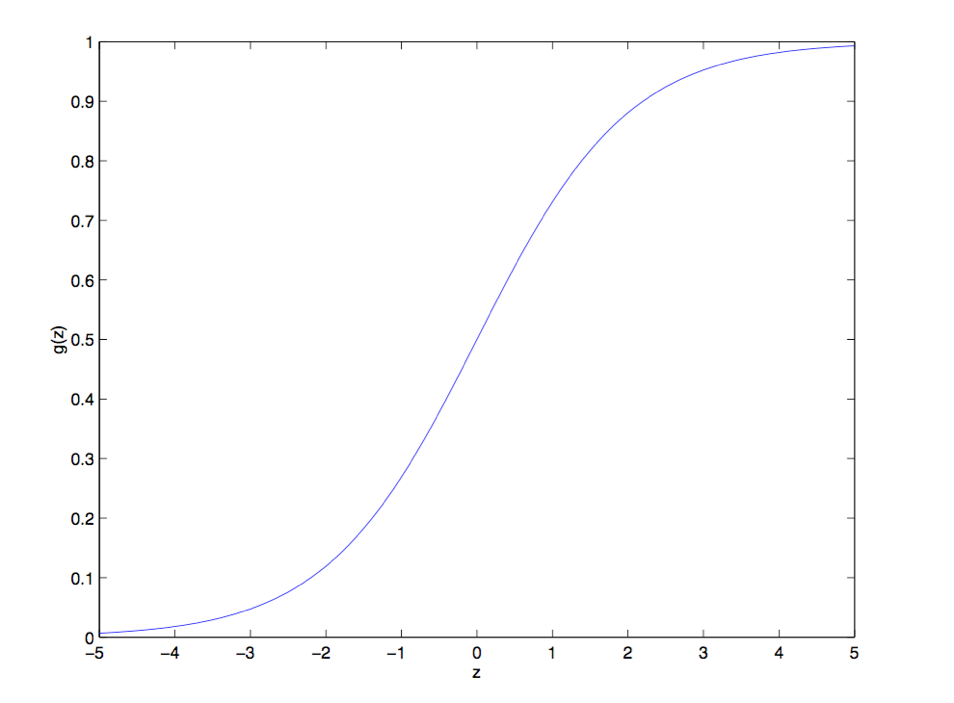
\includegraphics[height=7cm]{\pathroot/theory/lr/images/sigmoid.png}

\section{Logistic回归}
这一章用来介绍常用的线性模型,主要包括:多元线性回归、Logistic回归(LR)。

\subsection{mnist数据集简介}


%$\left(
%  \begin{array}{cccccccccccccccccccccccccccc}
%        0 & 0 & 0 & 0 & 0 & 0 & 0 & 0 & 0 & 0 & 0 & 0 & 0 & 0 & 0 & 0 & 0 & 0 & 0 & 0 & 0 & 0 & 0 & 0 & 0 & 0 & 0 & 0\\
%        0 & 0 & 0 & 0 & 0 & 0 & 0 & 0 & 0 & 0 & 0 & 0 & 0 & 0 & 0 & 0 & 0 & 0 & 0 & 0 & 0 & 0 & 0 & 0 & 0 & 0 & 0 & 0\\
%        0 & 0 & 0 & 0 & 0 & 0 & 0 & 0 & 0 & 0 & 0 & 0 & 0 & 0 & 0 & 0 & 0 & 0 & 0 & 0 & 0 & 0 & 0 & 0 & 0 & 0 & 0 & 0\\
%        0 & 0 & 0 & 0 & 0 & 0 & 0 & 0 & 0 & 0 & 0 & 0 & 0 & 0 & 0 & 0 & 0 & 0 & 0 & 0 & 0 & 0 & 0 & 0 & 0 & 0 & 0 & 0\\
%        0 & 0 & 0 & 0 & 0 & 0 & 0 & 0 & 0 & 0 & 0 & 0 & 0 & 0 & 0 & 0 & 0 & 0 & 0 & 0 & 0 & 0 & 0 & 0 & 0 & 0 & 0 & 0\\
%        0 & 0 & 0 & 0 & 0 & 0 & 0 & 0 & 0 & 0 & 0 & 0 & 3 & 18 & 18 & 18 & 126 & 136 & 175 & 26 & 166 & 255 & 247 & 127 & 0 & 0 & 0 & 0\\
%        0 & 0 & 0 & 0 & 0 & 0 & 0 & 0 & 30 & 36 & 94 & 154 & 170 & 253 & 253 & 253 & 253 & 253 & 225 & 172 & 253 & 242 & 195 & 64 & 0 & 0 & 0 & 0\\
%        0 & 0 & 0 & 0 & 0 & 0 & 0 & 49 & 238 & 253 & 253 & 253 & 253 & 253 & 253 & 253 & 253 & 251 & 93 & 82 & 82 & 56 & 39 & 0 & 0 & 0 & 0 & 0\\
%        0 & 0 & 0 & 0 & 0 & 0 & 0 & 18 & 219 & 253 & 253 & 253 & 253 & 253 & 198 & 182 & 247 & 241 & 0 & 0 & 0 & 0 & 0 & 0 & 0 & 0 & 0 & 0\\
%        0 & 0 & 0 & 0 & 0 & 0 & 0 & 0 & 80 & 156 & 107 & 253 & 253 & 205 & 11 & 0 & 43 & 154 & 0 & 0 & 0 & 0 & 0 & 0 & 0 & 0 & 0 & 0\\
%        0 & 0 & 0 & 0 & 0 & 0 & 0 & 0 & 0 & 14 & 1 & 154 & 253 & 90 & 0 & 0 & 0 & 0 & 0 & 0 & 0 & 0 & 0 & 0 & 0 & 0 & 0 & 0\\
%        0 & 0 & 0 & 0 & 0 & 0 & 0 & 0 & 0 & 0 & 0 & 139 & 253 & 190 & 2 & 0 & 0 & 0 & 0 & 0 & 0 & 0 & 0 & 0 & 0 & 0 & 0 & 0\\
%        0 & 0 & 0 & 0 & 0 & 0 & 0 & 0 & 0 & 0 & 0 & 11 & 190 & 253 & 70 & 0 & 0 & 0 & 0 & 0 & 0 & 0 & 0 & 0 & 0 & 0 & 0 & 0\\
%        0 & 0 & 0 & 0 & 0 & 0 & 0 & 0 & 0 & 0 & 0 & 0 & 35 & 241 & 225 & 160 & 108 & 1 & 0 & 0 & 0 & 0 & 0 & 0 & 0 & 0 & 0 & 0\\
%        0 & 0 & 0 & 0 & 0 & 0 & 0 & 0 & 0 & 0 & 0 & 0 & 0 & 81 & 240 & 253 & 253 & 119 & 25 & 0 & 0 & 0 & 0 & 0 & 0 & 0 & 0 & 0\\
%        0 & 0 & 0 & 0 & 0 & 0 & 0 & 0 & 0 & 0 & 0 & 0 & 0 & 0 & 45 & 186 & 253 & 253 & 150 & 27 & 0 & 0 & 0 & 0 & 0 & 0 & 0 & 0\\
%        0 & 0 & 0 & 0 & 0 & 0 & 0 & 0 & 0 & 0 & 0 & 0 & 0 & 0 & 0 & 16 & 93 & 252 & 253 & 187 & 0 & 0 & 0 & 0 & 0 & 0 & 0 & 0\\
%        0 & 0 & 0 & 0 & 0 & 0 & 0 & 0 & 0 & 0 & 0 & 0 & 0 & 0 & 0 & 0 & 0 & 249 & 253 & 249 & 64 & 0 & 0 & 0 & 0 & 0 & 0 & 0\\
%        0 & 0 & 0 & 0 & 0 & 0 & 0 & 0 & 0 & 0 & 0 & 0 & 0 & 0 & 46 & 130 & 183 & 253 & 253 & 207 & 2 & 0 & 0 & 0 & 0 & 0 & 0 & 0\\
%        0 & 0 & 0 & 0 & 0 & 0 & 0 & 0 & 0 & 0 & 0 & 0 & 39 & 148 & 229 & 253 & 253 & 253 & 250 & 182 & 0 & 0 & 0 & 0 & 0 & 0 & 0 & 0\\
%        0 & 0 & 0 & 0 & 0 & 0 & 0 & 0 & 0 & 0 & 24 & 114 & 221 & 253 & 253 & 253 & 253 & 201 & 78 & 0 & 0 & 0 & 0 & 0 & 0 & 0 & 0 & 0\\
%        0 & 0 & 0 & 0 & 0 & 0 & 0 & 0 & 23 & 66 & 213 & 253 & 253 & 253 & 253 & 198 & 81 & 2 & 0 & 0 & 0 & 0 & 0 & 0 & 0 & 0 & 0 & 0\\
%        0 & 0 & 0 & 0 & 0 & 0 & 18 & 171 & 219 & 253 & 253 & 253 & 253 & 195 & 80 & 9 & 0 & 0 & 0 & 0 & 0 & 0 & 0 & 0 & 0 & 0 & 0 & 0\\
%        0 & 0 & 0 & 0 & 55 & 172 & 226 & 253 & 253 & 253 & 253 & 244 & 133 & 11 & 0 & 0 & 0 & 0 & 0 & 0 & 0 & 0 & 0 & 0 & 0 & 0 & 0 & 0\\
%        0 & 0 & 0 & 0 & 136 & 253 & 253 & 253 & 212 & 135 & 132 & 16 & 0 & 0 & 0 & 0 & 0 & 0 & 0 & 0 & 0 & 0 & 0 & 0 & 0 & 0 & 0 & 0\\
%        0 & 0 & 0 & 0 & 0 & 0 & 0 & 0 & 0 & 0 & 0 & 0 & 0 & 0 & 0 & 0 & 0 & 0 & 0 & 0 & 0 & 0 & 0 & 0 & 0 & 0 & 0 & 0\\
%        0 & 0 & 0 & 0 & 0 & 0 & 0 & 0 & 0 & 0 & 0 & 0 & 0 & 0 & 0 & 0 & 0 & 0 & 0 & 0 & 0 & 0 & 0 & 0 & 0 & 0 & 0 & 0\\
%        0 & 0 & 0 & 0 & 0 & 0 & 0 & 0 & 0 & 0 & 0 & 0 & 0 & 0 & 0 & 0 & 0 & 0 & 0 & 0 & 0 & 0 & 0 & 0 & 0 & 0 & 0 & 0
%    \end{array}
%\right)$

\subsection{Logistic Regression}

\begin{itemize}
\item logistic函数/sigmoid函数: $h_{\theta}(x)=g({\theta}^Tx)={\frac {1}{1+e^{-\theta^Tx}}}$ 
\item 函数可导:
$g'(z)={\frac {d}{dz}}{\frac {1}{1+e^{-\theta^Tx}}}=\lim_{{\Delta x}\to 0}{\frac {f(x+{\Delta x})-f(x)}{\Delta x}}$
\end{itemize}

\begin{itemize}
\item 对于一个二分类问题,可假设$h_{\theta}(x)$为其中一类的概率,即:
\subitem $P(y=1|x;\theta)=h_{\theta}(x)$
\subitem $P(y=0|x;\theta)=1-h_{\theta}(x)$
\item 更简洁的形式: $P(y|x;\theta)={h_{\theta}(x)}^y(1-h_{\theta}(x))^{1-y}$
\item 假设$m$个训练样本独立,则样本集在参数${\theta}$给定下,出现的概率为:

\item 我们希望最大化概率$L({\theta})$,也即最大化log似然值:

\item 最大化一个目标值,可采用梯度上升法,沿着梯度方向不断迭代。梯度求解如下:

\item 随机梯度下降法求解:
\subitem ${\theta}_{j}:={\theta}_{j}+{\alpha}(y^{(i)}-h_{\theta}(x^{(i)}))x_{j}^{(i)}$

\item 思考:
\subitem 如果引入$L1$正则、$L2$正则,那么梯度又该怎么求解呢?
\subitem LR的梯度求解公式与线性回归的梯度求解公式看起来一样,有区别么?

\item L1:$cost(w)={\frac {1}{2m}}\left\|{Xw-y}\right\|^{2}+\lambda\|w\|_{1}$
,等价于
    $\min\limits_{w}{\frac {1}{2m}}\left\|{Xw-y}\right\|^{2}, s.t. \left\|w\right\|_{1}\le{C}$

\item L2:$cost(w)={\frac {1}{2m}}\left\|{Xw-y}\right\|^{2}+{\frac {\lambda}{2}}\|w\|_{2}^{2}$
,等价于
    $\min\limits_{w}{\frac {1}{2m}}\left\|{Xw-y}\right\|^{2}, s.t. \left\|w\right\|_{2}^{2}\le{C}$

\item 常用分类器的评价指标有:准确率(precision)、召回率(recall)、F值、正确率(accuracy)等
\end{itemize}

\begin{itemize}

\item 考虑ROC曲线图中的四个点。
    \subitem(1)第一个点(0,1),FPR=0, TPR=1,即FN=0,并且FP=0。
        \subsubitem 特点:正确分类所有的样本。
    \subitem(2)第二个点(1,0),FPR=1,TPR=0。
        \subsubitem 特点:成功错分了所有的样例。
    \subitem(3)第三个点(0,0),FPR=TPR=0,即FP=TP=0,
        \subsubitem 特点:分类器预测所有的样本都为负样本。
    \subitem(4)第四个点(1,1),分类器预测所有的样本都为正样本。
\item 结论:ROC曲线越接近左上角,该分类器的性能越好。
\item 考虑ROC曲线图中的虚线$y=x$上的点。这条对角线上的点表示的是一个采用随机猜测策略的分类器的结果。

\item ROC曲线的画法:对一个特定的测试数据集合,对分类模型输出的概率值设置不同的阈值,从而得到一组(FPR,TPR)点,以此连接这些点即可得到ROC曲线。
\item AUC(Area Under Curve):ROC曲线下的面积。
\item AUC值等于一个随机选择的正样本的预测值高于一个随机选择的负样本的概率。
\item ROC曲线的优点:当测试集中的正负样本的分布变化的时候,ROC曲线能够保持不变。

\item 在右图中,(a)和(c)为ROC曲线,(b)和(d)为\\
Precision-Recall曲线。(a)和(b)展示的是\\
分类其在原始测试集(正负样本分布平衡)\\
的结果,(c)和(d)是将测试集中负样本的数\\
量增加到原来的10倍后, 分类器的结果。可\\
以明显的看出,ROC曲线基本保持原貌,\\
而Precision-Recall曲线则变化较大。

\item 基本思路:将多分类任务拆若干个二分类任务。学习时分别训练多个分类器,测试时对这多个分类器的预测结果进行集成以获得最终的多分类结果
\item 一对一(OvO) 
    \subitem 以$C_{i}$与$C_{j}$的数据作为正反例训练一个分类器,共训练${\frac {N(N-1)}{2}}$个分类器
    \subitem 预测时将样本提交给所有分类器,获取${\frac {N(N-1)}{2}}$个结果,最终结果通过投票产生
\item 一对多(OvR)
    \subitem 以$C_{i}$数据为正例,其余类别数据为负例,训练$N$个分类器
\item 其他:如多对多(MvM)策略的ECOC编码
\end{itemize}

\section{Softmax Regression}
这一章用来介绍常用的线性模型,主要包括:多元线性回归、Logistic回归(LR)。

\subsection{Softmax Regression}

\begin{itemize}
\item 简介:为LR在多分类上的推广。与LR一样,同属于广义线性模型(Generalized Linear Model)。
\item $P(y=i|x;{\theta})={\frac {e^{{\theta}_{i}^{T}x}}{\sum_{j=1}^{K}{e^{{\theta}_{j}^{T}x}}}}$
\item 同样,考虑使得对数似然最大,则系统损失函数为:\\
    $\ell(\theta)=-{\frac {1}{m}}\left[\sum\limits_{i=1}^{m}{\sum\limits_{j=1}^{K}{1\{y^{(i)}=j\}\log{\frac{e^{{\theta}_{j}^{T}{x^{(i)}}}}{\sum_{l=1}^{K}{e^{\theta_{l}^{T}x^{(i)}}}}}}}\right]$
\item 加入正则项:\\
    $\ell(\theta)=-{\frac {1}{m}}\left[\sum\limits_{i=1}^{m}{\sum\limits_{j=1}^{K}{1\{y^{(i)}=j\}\log{\frac{e^{{\theta}_{j}^{T}{x^{(i)}}}}{\sum_{l=1}^{K}{e^{\theta_{l}^{T}x^{(i)}}}}}}}\right]+
    {\frac {\lambda}{2}{\sum\limits_{i=1}^{K}{\sum\limits_{j=0}^{n}{\theta_{ij}^{2}}}}}$

\item 考虑一个样本$(x,y)$,有$\ell(x,\hat{y})=-\sum\limits_{j=1}^{K}{1\{y=j\}\ln{\hat{y}_{j}}}$,令$a_{j}={\theta_{j}^{T}x}$,有
\begin{align*}
{\frac {\partial \ell(x,\hat{y})}{a_{j}}}&=\sum\limits_{i=1}^{K}{{\frac {\partial \ell(x,\hat{y})}{\partial \hat{y}_{i}}}{\frac {\partial \hat{y}_{i}}{\partial a_{j}}}}\\
                                         &=-\sum\limits_{i=1}^{K}{
                                                {\frac {1\{y=i\}}{\hat{y}_{i}}}
                                                {\frac {\partial \frac {e^{a_{i}}}{\sum_{l=1}^{K}{e^{a_{l}}}}}{\partial a_{j}}}}\\
                                         &=-\sum\limits_{i=1}^{K}{
                                                {\frac {1\{y=i\}}{\hat{y}_{i}}}
                                                {\frac {
                                                            e^{a_{i}} \cdot 1\{i=j\} \cdot {\left({\sum_{l=1}^{K}{e^{a_{l}}}}\right)}
                                                            -e^{a_{i}} \cdot e^{a_{j}}
                                                        }
                                                       {\left({\sum_{l=1}^{K}{e^{a_{l}}}}\right)^{2}}
                                                    }}\\
                                         &=\sum\limits_{i=1}^{K}{
                                                {\frac {1\{y=i\}}{\hat{y}_{i}}}
                                                {\frac {e^{a_{i}} \cdot e^{a_{j}}}
                                                       {\left({\sum_{l=1}^{K}{e^{a_{l}}}}\right)^{2}}
                                                    }}
                                            -\sum\limits_{i=1}^{K}{
                                                {\frac {1\{y=i\}}{\hat{y}_{i}}}
                                                {\frac {e^{a_{i}} \cdot 1\{i=j\} \cdot {\left({\sum_{l=1}^{K}{e^{a_{l}}}}\right)}}
                                                       {\left({\sum_{l=1}^{K}{e^{a_{l}}}}\right)^{2}}
                                                    }}\\
                                         &=\sum\limits_{i=1}^{K}{{\frac {1\{y=i\}}{\hat{y}_{i}}}{\hat{y}_{i}}{\hat{y}_{j}}}
                                            -\sum\limits_{i=1}^{K}{{\frac {1\{y=i\}}{\hat{y}_{i}}}{\hat{y}_{i}} \cdot 1\{i=j\}}\\
                                         &={\hat{y}_{j}}-\sum\limits_{i=1}^{K}{{1\{y=i\}}} \cdot 1\{i=j\}\\
                                         &={\hat{y}_{j}}-{1\{y=j\}} \\
\end{align*}


\item 如果待分的类别互斥,使用softmax
\item 如果类别有交叉,则使用LR进行投票分类
\item 例如
    \subitem 有四个类别的音乐,分别为:古典音乐、乡村音乐、摇滚乐和爵士乐
    \subitem 有四个类别如下:人声音乐、舞曲、影视原声、流行歌曲


\item 实际工程中,LR很少使用连续特征。一般将连续特征离散化成多个取值为0/1的离散特征。
\subitem 0. 离散特征的增加和减少都很容易,易于模型的快速迭代;
\subitem 1. 稀疏向量内积乘法运算速度快,计算结果方便存储,容易扩展;
\subitem 2. 离散化后的特征对异常数据有很强的鲁棒性;
\subitem 3. 逻辑回归属于广义线性模型,表达能力受限;离散化相当于为模型引入了非线性,提升模型表达能力;
\subitem 4. 离散化后可以进行特征交叉,由$M+N$个变量变为$M*N$个变量,进一步引入非线性,提升表达能力;
\subitem 5. 特征离散化后,模型会更稳定;
\subitem 6. 特征离散化以后,起到了简化了逻辑回归模型的作用,降低了模型过拟合的风险。

\end{itemize}




\begin{itemize}
\item 监督学习:利用一组已知类别的样本调整分类器的参数,\\使其达到所要求性能的过程
\item 一些符号定义:

$x^{(i)}$:指数据集中的第$i$个样本的特征类数据。

$y^{(i)}$:指数据集中的第$i$个样本的目标值。

$\left(x^{(i)},y^{(i)}\right)$:表示一个样本实例。

$\left\{\left(x^{(i)},y^{(i)}\right), i=1,...,N\right\}$:表示一个数据集。
\\例如,对于手写体识别来说,图片的像素表示即为特征$x$,图片表示的数字即为目标值$y$。

\end{itemize}

对于红酒问题,
\begin{itemize}
\item 问题分析:
\\(1) 共有11个特征,可表示为11个变量:$x^{(i)}_1,x^{(i)}_2,...,x^{(i)}_{11}$。
\\(2) 目标只有一个评分,可表示为:$y^{(i)}$
\\(3) 问题可表示为优化问题:$argmin_{w}\sum_{i=1}^{N}(w_0 + w_1*x^{(i)}_1 + w_2*x^{(i)}_2 + w_{11}*x^{(i)}_{11} - y^{(i)})^2$

\item 用向量表示更加简洁:
\\(1) 特征表示为:$x^{(i)}=\left(\begin{array}{ccc}x^{(i)}_0,x^{(i)}_1,...,x^{(i)}_{11}\end{array}\right)^T$,其中$x^{(i)}_0=1$
\\(2) 权重系数表示为:$w=\left(\begin{array}{ccc}w_0,w_1,...,w_{11}\end{array}\right)^T$
\\(3) 问题表示为:$argmin_{w} \sum_{i=1}^{N}(w^Tx^{(i)}-y^{(i)})^2$

\end{itemize}

\begin{equation}
  s_{kk'}=
  \left(
  \begin{array}{ccc}
          h_{1k} &
          \cdots &
          h_{nk}
  \end{array}
  \right)
  \left(
  \begin{array}{ccc}
          \bar{q}_{11} & \cdots & \bar{q}_{12}\\
          \vdots & \ddots & \vdots\\
          \bar{q}_{n1} & \cdots & \bar{q}_{n2}
  \end{array}
  \right)
  \left(
  \begin{array}{c}
          h_{1k'} \\
          \vdots \\
          h_{nk'}
 \end{array}
 \right)
\end{equation}


%\\$x=\begin{matrix} 0 & 1 \end{matrix}$

\subsubsection{Linear Regression}
\begin{itemize}

\item 给定一份数据集$\left\{x_0^{(i)},x_1^{(i)},...,x_m^{(i)},y^{(i)}\right\}_{i=0}^{N-1}$,线性回归假设目标值$y^{(i)}$与特征$x^{(i)}$之间为线性关系,即:$$y^{(i)}=w_0x_0^{(i)}+w_1x_1^{(i)}+...+w_mx_m^{(i)}$$

\item 现实世界不存在完美线性相关的关系,总会有各\\
种各样的偏差存在。由大数定理,可假设真实值\\
总在理论值附近波动,误差符合高斯分布, 即:\\
$y^{(i)}=w_0x_0^{(i)}+w_1x_1^{(i)}+...+w_mx_m^{(i)}+\varepsilon^{(i)}$\\
其中,$\varepsilon^{(i)}\sim{\mathcal{N}}(0, \sigma^{2})$
%其中,$\varepsilon\sim{\mathcal{N}}(\mu, \sigma^{2})$

\item 假设训练集中一共有$N$个样本:

$X=\left(
\begin{array}{c}
        {(x^{(0)})}^T \\
        {(x^{(1)})}^T \\
        \vdots \\
        {(x^{(N-1)})}^T \\
\end{array}
\right)=\left(
\begin{array}{ccc}
        x_0^{(0)} & \cdots & x_m^{(0)} \\
        x_0^{(1)} & \cdots & x_m^{(1)} \\
        \vdots & \ddots & \vdots\\
        x_0^{(N-1)} & \cdots & x_m^{(N-1)}
\end{array}
\right)$
$w=\left(
\begin{array}{c}
        w^{(0)} \\
        w^{(1)} \\
        \vdots \\
        w^{(m)}
\end{array}
\right)$
$y=\left(
\begin{array}{c}
        y^{(0)} \\
        y^{(1)} \\
        \vdots \\
        y^{(N-1)}
\end{array}
\right)$

\item 线性回归的目标就是最小化预估值与真实值的差距,也即所求$w$满足:$$argmin \left\|{Xw-y}\right\|^{2}$$
\item 代数解:$w=(X^{T}X)^{-1}X^{T}y$
\end{itemize}


\begin{itemize}
\item 代数解非常优美:\\
(1) 当$X^{T}X$为满秩矩阵或正定矩阵时,上式有唯一解。\\
(2) 现实任务中往往不是满秩矩阵,即$X^{T}X$不可逆,原因有很多,例如:
    \begin{itemize}
    \item 存在冗余特征,例如特征之间相关
    \item 训练样本少,如特征数甚至超过样本数
    \end{itemize}
此时$w$有多个可行解,需要选择最佳$w$。 \\
(3) 此代数解运算复杂度高,当$n>10000$时开销过大。\\

\end{itemize}

\subparagraph{梯度下降}
介绍梯度下降的原理。
\subsection{理论}

\begin{itemize}
\item 想法:人类在学习的时候,都是渐进式学习,不断从错误中纠正自己的认知,从而越来越优秀。
\item 导数定义:$ {\frac {dy}{dx}}={\frac {df}{dx}}(x)={\frac {d}{dx}}f(x)=f'(x)=\lim_{{\Delta x}\to 0}{\frac {f(x+{\Delta x})-f(x)}{\Delta x}} $\\
有:$f(x+{\Delta x})-f(x)=f'(x){\Delta x}$
\\(1) 如果$f'(x)>0$:
\subitem 当${\Delta x}>0$时,$f(x+{\Delta x})-f(x)=f'(x){\Delta x}>0$;
\subitem 当${\Delta x}<0$时,$f(x+{\Delta x})-f(x)=f'(x){\Delta x}<0$
\\(2) 如果$f'(x)<0$:
\subitem 当${\Delta x}>0$时,$f(x+{\Delta x})-f(x)=f'(x){\Delta x}<0$;
\subitem 当${\Delta x}<0$时,$f(x+{\Delta x})-f(x)=f'(x){\Delta x}>0$
\item 结论:如果使$x$变化的方向与$f'(x)$一致,将会使得$f(x)$增加。
\end{itemize}

\begin{itemize}
\item 梯度:$\nabla f=\left({\frac {\partial f}{\partial x_{1}}},\dots ,{\frac {\partial f}{\partial x_{n}}}\right)$,其中$\left(\nabla f\right)_{i}={\frac {\partial f}{\partial x_{i}}}$
\item 梯度下降算法(Gradient Descent):沿梯度下降的方向求解极小值。
\item 算法过程:
\\(1) 初始化参数为任意值。例如线性回归中的$w$。
\\(2) 求解梯度。例如线性回归中,求解 $\nabla\left(\left\|{Xw-y}\right\|^{2}\right)$。
\\(3) 更新参数。例如线性回归中,更新参数$w$,\\使得$w=w-\alpha\nabla\left(\left\|{Xw-y}\right\|^{2}\right)$,$\alpha$称为学习率。
\\(4) 若达到指定迭代次数或者收敛条件,训练结束。\\否则,继续执行步骤(2)。
\end{itemize}

\begin{itemize}
\item 实际应用中,对梯度下降算法有很多变形或改进。
\item 随机梯度下降(stochastic gradient descent):每遇到
\\一个或者多个但不是整个样本集,就计算梯度,更新参数。
\item 算法过程:
\\(1) 初始化参数为任意值。例如线性回归中的$w$。
\\(2) 对样本集中的每个样本,做如下操作直接完成所有样本\\的遍历:
\subitem(2.1) 求解梯度。例如线性回归中,求解 $\nabla\left(\left\|{Xw-y}\right\|^{2}\right)$。
\subitem(2.2) 更新参数。例如线性回归中,更新参数$w$,使得$w=w-\alpha\nabla\left(\left\|{Xw-y}\right\|^{2}\right)$。
\\(3) 若达到指定迭代次数或者收敛条件,训练结束。否则,继续执行步骤(2)。
\end{itemize}

\begin{itemize}
\item 一个完整的有监督学习的开发流程:
\\(1) 获取数据,对数据做一些清洗、转换等操作。
\\(2) 将数据样本拆分成训练集、验证集和测试集。训练集用来训练模型,验证集用来评估模型效果和调参,测试集则用来评估最终的模型效果。
\\(3) 开发模型或直接使用开发好的模型工具,在训练集上进行训练。
\\(4) 获取训练好的模型,使用验证集评估其效果。如果没有达到预期,需要进一步对模型调参、获取新的特征等操作,直到满足训练效果为止。
\\(5) 使用训练好的模型,在测试集上评估其最终效果。

\item 对于葡萄酒质量预估任务来说,主要有以下过程(只使用白酒的数据):
\\(1) 获取数据集,对数据集做一些预处理操作。
\\(2) 将处理好的数据集分为训练集、验证集和测试集,比例为:0.7:0.2:0.1。
\\(3) 开发线性回归模型。
\\(4) 在训练集上训练线性模型,在验证集上验证模型效果。没有达到预期,需要调参,直到满足训练效果为止。
\\(5) 在测试集中获取最终效果。

\end{itemize}

$x'={\frac {x - x_{min}}{x_{max} - x_{min}}}$

\begin{itemize}
\item 正则项:为有效控制模型参数的复杂度,加入参数复杂度的惩罚项,以使得模型选择更加简单的参数。
\item L1正则:$cost(w)={\frac {1}{2N}}\left\|{Xw-y}\right\|^{2}+\lambda\|w\|_{1}$
\item L2正则:$cost(w)={\frac {1}{2N}}\left\|{Xw-y}\right\|^{2}+{\frac {\lambda}{2}}\|w\|_{2}^{2}$
\\

加入正则项后,梯度:
\item L1正则:$w=w-\alpha (w^{T}x^{(i)}-y^{(i)})x^{(i)} - \alpha\lambda w$
\item L2正则:$w=w-\alpha (w^{T}x^{(i)}-y^{(i)})x^{(i)} - \alpha\lambda sign(w)$
\end{itemize}

\begin{itemize}
\item 优化目标:$cost(w)={\frac {1}{2N}}\left\|{Xw-y}\right\|^{2}$
\item 对于单个样本来说:$cost(w)={\frac {1}{2}}\left({w^{T}x^{(i)}-y^{(i)}}\right)^{2}$
\item 单个样本的梯度为:$\nabla cost(w)=(w^{T}x^{(i)}-y^{(i)})x^{(i)}$
\item 梯度更新:$w=w-\alpha (w^{T}x^{(i)}-y^{(i)})x^{(i)}$
\item 样本特征的取值情况如右图所示
\item 特征归一化: $x'={\frac {x - x_{min}}{x_{max} - x_{min}}}$

\end{itemize}

\subsection{交叉验证{\color{red} TODO}}

交叉验证(Cross Validation),有的时候也称作循环估计(Rotation Estimation),是一种统计学上将数据样本切割成较小子集的实用方法,该理论是由Seymour Geisser提出的。

在模式识别(Pattern Recognition)和机器学习(Machine Learning)的相关研究中,经常会将整个数据集合分成两个部分,分别是训练集合和测试集合。假设X是集合全体,A是全集X的非空真子集,那么非空集合X\textbackslash{A}则是集合A在全集X中的补集。于是可以先在A上面做训练和分析,而集合X\textbackslash{A}则用来做测试和验证。一开始的集合A被称作训练集,而它的补集X\textbackslash{A}被称作验证集或者测试集。这里有一个重要的观点就是:只有训练集才可以使用在模型的训练之中,而测试集必须在模型训练完成之后才被用来评估模型的误差。

\subsubsection{HoldOut检验(Hold-Out Method)}
这个方法是将原始的数据集合X随机分成两个集合A和X\textbackslash{A},其中A作为训练集,X\textbackslash{A}作为测试集。先使用训练集训练模型,然后利用测试集验证模型的效果,记录最后的分类准确率作为Hold-Out下该模型的性能指标。比方说,处理时间序列模型是否准确的时候,把整个数据集合分成前后两部分,前部分占比70\%,后部分占比30\%。前部分来进行时间序列模型的训练,后部分用来测试改时间序列的准确性。其准确性可以用MAE,MAPE之类的统计指标来衡量。综上所述,该方法的好处就是处理起来简单,只需要把原始数据分成两个部分即可。但是从严格意义上来说,Hold-Out检验并不算是交叉检验(Cross Validation),因为该方法没有达到交叉检验的思想,而且最后验证准确性的高低和原始数组的分类有很大的关系,所以该方法得到的结果在某些场景中并不具备特别大的说服力。在Hold-Out检验不够有说服力的情形下,有人提出了交叉验证这一个重要思想。

\textbf{testing中文}
\bf{testing中文}

\subsubsection{交叉检验的常见形式}
假设有一个未知模型有一个或者多个未知的参数,并且有一个训练集。操作的过程就是对该模型的参数进行调整,使得该模型能够最大的反映训练集的特征。如果模型因为训练集过小或者参数不合适而产生过度拟合的情况,测试集的测试效果就可以得到验证。交叉验证是一种能够预测模型拟合性能的有效方法。

\subsubsection{彻底的交叉验证(Exhaustive Cross Validation)}
彻底的交叉验证方法指的是遍历全集X的所有非空真子集A。换句话说也就是把A当作训练集,X\textbackslash{A}是测试集。如果X中有n个元素,那么非空真子集A的选择方法则是$2^{n}-2$,这个方法的时间复杂度是指数级别的。

\begin{itemize}
\item 留P验证(Leave-p-out Cross Validation)
留p验证(LpO CV)指的是使用全集X中的p个元素作为测试集,然后剩下的n-p个元素作为训练集。根据数学上的定理可以得到,p个元素的选择方法有n!/((n-p)!p!)个,其中n!表示n的阶乘。在这个意义下,留p验证的时间复杂度也是非常高的。当p=1的时候,留1验证(Leave-one-out Cross Validation)的复杂度恰好是n。

\item 不彻底的交叉验证(Non-exhaustive Cross Validation)
不彻底的交叉验证不需要考虑全集X的所有划分情况,这种方法是留p验证的一个近似验证算法。

\item k-fold交叉验证(K-fold Cross Validation)
在k-fold交叉验证中,全集X被随机的划分成k个同等大小的集合A1,...,Ak,并且|A1|=...=|Ak|。这里的|Ai|指的是集合Ai的元素个数,也就是集合的势。这个时候需要遍历i从1到k,把X\textbackslash{Ai}当作训练集合,Ai当作测试集合。根据模型的测试统计,可以得到Ai集合中测试错误的结果数量ni。如果全集X的势是n的话,可以得到该模型的错误率是E=(ni求和)/n.
为了提高模型的精确度,可以将k-fold交叉验证的上述步骤重复t次,每一次都是随机划分全集X。在t次测试中,会得到t个模型的错误率E1,...,Et。令e=(Ei求和)/t。这样该模型的错误率就是e。

注释:
一般来说,k=10的情况使用得最多。
当k=2的时候,也就是最简单的k-fold交叉验证,2-fold交叉验证。这个时候X是A1和A2的并集,首先A1当训练集并且A2当测试集,然后A2当训练集并且A1当测试集。2-fold交叉验证的好处就是训练集和测试集的势都非常大,每个数据要么在训练集中,要么在测试集中。
当k=n的时候,也就是n-fold交叉验证。这个时候就是上面所说的留一验证(Leave-one-out Cross Validation)。
\end{itemize}
综上所述,交叉验证(Cross Validation)的好处是可以从有限的数据中获得尽可能多的有效信息,从而可以从多个角度去学习样本,避免陷入局部的极值。在这个过程中,无论是训练样本还是测试样本都得到了尽可能多的学习。

一般模型的选择过程:
在了解了交叉验证的方法之后,可以来介绍一般模型的选择过程。通过采用不同的输入训练样本,来决定机器学习算法中包含的各个参数值,称作模型选择。下面伪代码表示了模型选择的一般流程。在这个算法中,最重要的就是第三个步骤中的误差评价。 
(1)准备候选的q个模型:M1,...,Mq。 
(2)对每个模型M1,...,Mq求解它的学习结果。 
(3)对每个学习结果的误差e1,...,eq进行计算。这里可以使用上面所说的k-fold交叉验证方法。 
(4)选择误差e1,...,eq最小的模型作为最终的模型。









交叉验证是一种用来评价一个统计分析的结果是否可以推广到一个独立的数据集上的技术。主要用于预测,即,想要估计一个预测模型的实际应用中的准确度。它是一种统计学上将数据样本切割成较小子集的实用方法。于是可以先在一个子集上做分析, 而其它子集则用来做后续对此分析的确认及验证。 

交叉验证的理论是由Seymour Geisser所开始的。 它对于防范testing hypotheses suggested by the data是非常重要的,特别是当后续的样本是危险、成本过高或不可能(uncomfortable science)去搜集。

一个交叉验证将样本数据集分成两个互补的子集,一个子集用于训练(分类器或模型)称为训练集(training set);另一个子集用于验证(分类器或模型的)分析的有效性称为测试集(testing set)。利用测试集来测试训练得到的分类器或模型,以此作为分类器或模型的性能指标。

得到高度预测精确度和低的预测误差,是研究的期望。为了减少交叉验证结果的可变性,对一个样本数据集进行多次不同的划分,得到不同的互补子集,进行多次交叉验证。取多次验证的平均值作为验证结果。

在给定的建模样本中,拿出大部分样本进行建模型,留小部分样本用刚建立的模型进行预报,并求这小部分样本的预报误差,记录它们的平方加和。这个过程一直进行,直到所有的样本都被预报了一次而且仅被预报一次。把每个样本的预报误差平方加和,称为PRESS(predicted Error Sum of Squares)。

\subsubsection{目的}
用交叉验证的目的是为了得到可靠稳定的模型。在建立PCR 或PLS 模型时,一个很重要的因素是取多少个主成分的问题?用cross validation 校验每个主成分下的PRESS值,选择PRESS值小的主成分数。或PRESS值不在变小时的主成分数

交叉验证的目的:假设分类器或模型有一个或多个未知的参数,并且设这个训练器(模型)与已有样本数据集(训练数据集)匹配。训练的过程是指优化模型的参数,以使得分类器或模型能够尽可能的与训练数据集匹配。我们在同一数据集总体中,取一个独立的测试数据集。
\subsubsection{常见类型的交叉验证}
\begin{itemize}
\item 重复随机子抽样验证。
    \subitem 做法:将数据集随机的划分为训练集和测试集。对每一个划分,用训练集训练分类器或模型,用测试集评估预测的精确度。进行多次划分,用均值来表示效能。
    \subitem 优点:与k倍交叉验证相比,这种方法的与k无关。
    \subitem 缺点:有些数据可能从未做过训练或测试数据;而有些数据不止一次选为训练或测试数据。
\item 2、K倍交叉验证(K>=2)。
    \subitem 做法:将样本数据集随机划分为K个子集(一般是均分),将一个子集数据作为测试集,其余的K-1组子集作为训练集;将K个子集轮流作为测试集,重复上述过程,这样得到了K个分类器或模型,并利用测试集得到了K个分类器或模型的分类准确率。用K个分类准确率的平均值作为分类器或模型的性能指标。10-倍交叉证实是比较常用的。
    \subitem 优点:每一个样本数据都即被用作训练数据,也被用作测试数据。避免的过度学习和欠学习状态的发生,得到的结果比较具有说服力。
\item 3、留一法交叉验证。
    \subitem 做法:假设样本数据集中有N个样本数据。将每个样本单独作为测试集,其余N-1个样本作为训练集,这样得到了N个分类器或模型,用这N个分类器或模型的分类准确率的平均数作为此分类器的性能指标。
    \subitem 优点:每一个分类器或模型都是用几乎所有的样本来训练模型,最接近样本,这样评估所得的结果比较可靠。实验没有随机因素,整个过程是可重复的。
    \subitem 缺点:计算成本高,当N非常大时,计算耗时。
\end{itemize}

\subsubsection{训练集和测试集的选取}
\begin{itemize}
\item 1、训练集中样本数量要足够多,一般至少大于总样本数的50%。
\item 2、训练集和测试集必须从完整的数据集中均匀取样。均匀取样的目的是希望减少训练集、测试集与原数据集之间的偏差。当样本数量足够多时,通过随机取样,便可以实现均匀取样的效果。(随机取样,可重复性差)
\end{itemize}

\subsection{Logistic Regression}

%\includegraphics[height=高度][angle=旋转角度]{图片文件名}
下面是一张图片

%\includegraphics[width=0.8\linewidth]{pic/logistic.png}

上面是一张图片

%\animategraphics[height=2.8in,autoplay,controls]{12}{pic/gradient.gif}{0}{39}


\ifx\mlbook\undefined
    \end{document}
\fi

\ifx\mlbook\undefined
    \documentclass[10pt,a4paper]{ctexbook}
    \providecommand{\pathroot}{../..}

    \usepackage[CJKbookmarks,colorlinks,linkcolor=red]{hyperref}
    \usepackage{geometry}
    \usepackage{amsmath}

    \geometry{left=3.0cm,right=3.0cm,top=2.5cm,bottom=2.5cm}
    \setmainfont{SimSun}
    \XeTeXlinebreaklocale "zh"
    \XeTeXlinebreakskip = 0pt plus 1pt minus 0.1pt

    \begin{document}
    \setlength{\baselineskip}{20pt}
    \title{Logistic回归}
    \author{Donald Cheung\\jianzhang9102@gmail.com}
    \date{Sep 8, 2017}
    \maketitle
    \tableofcontents
\fi

\chapter{神经网络}
\section{前馈神经网络}
Backpropagation Algorithm(BP算法)
\href{https://machinelearningmastery.com/implement-backpropagation-algorithm-scratch-python/}{How to Implement the Backpropagation Algorithm From Scratch In Python}

\section{RNN}
RNN理论基础,包括历史、类别、训练算法等。
\href{https://github.com/szcom/rnnlib}{rnnlib}



\subsection{BPTT}
\href{http://proceedings.mlr.press/v28/pascanu13.pdf}{On the difficulty of training recurrent neural networks}

\href{https://arxiv.org/abs/1211.5063}{On the difficulty of training recurrent neural networks}

\href{https://arxiv.org/abs/1606.03401}{Memory-Efficient Backpropagation Through Time}

\href{http://axon.cs.byu.edu/~martinez/classes/678/Papers/Werbos_BPTT.pdf}{Backpropagation Through Time: What It Does and How to Do It}

\href{https://arxiv.org/pdf/1406.1078v3.pdf}{Learning Phrase Representations using RNN Encoder-Decoder for Statistical Machine Translation}

\href{http://www.cs.utoronto.ca/~ilya/pubs/ilya_sutskever_phd_thesis.pdf}{Ilya Sutskever, Training Recurrent Neural Networks, Thesis, 2013}

\href{https://arxiv.org/abs/1503.04069}{LSTM: A Search Space Odyssey}

\href{https://arxiv.org/abs/1506.00019}{A Critical Review of Recurrent Neural Networks for Sequence Learning}

\href{https://jramapuram.github.io/ramblings/rnn-backrpop/}{BLOG: RNN Backprop Through Time Equations}

vanilla RNNs trained with BPTT \href{http://www.jmlr.org/proceedings/papers/v28/pascanu13.pdf}{have difficulties} learning long-term dependencies (e.g. dependencies between steps that are far apart) due to what is called the vanishing/exploding gradient problem. There exists some machinery to deal with these problems, and certain types of RNNs (like LSTMs) were specifically designed to get around them.

\[
\begin{aligned}
C_{i,j} & = -\tilde{P_{ij}} * o_{i,j} + log(1 + e^{o_{i,j}})\\o_{i,j} & = o_i - o_j\\\tilde{P_{i,j}} & = \{0, 0.5, 1\} \ or \ \{0, 1\}
\end{aligned}
\]

Cosine Similarity Layer. The cosine similarity equation is here.
\[similarity = cos(\theta) = {\mathbf{a} \cdot \mathbf{b} \over \|\mathbf{a}\| \|\mathbf{b}\|}\]
The size of a is M, size of b is M*N, Similarity will be calculated N times by step M. The output size is N. The scale will be multiplied to similarity.

Note that the above computation is for one sample. Multiple samples are processed in one batch.

\begin{table}[H]
\centering
\begin{tabular}{|l|l|l|}
\hline
Neural Layer & Description & Index variable\\
\hline
$x(t)$ & input layer & $i$ \\
$s(t-1)$ & previous hidden (state) layer & $h$ \\
$s(t)$ & hidden (state) layer & $j$ \\
$y(t)$ & output layer & $k$ \\
\hline
\end{tabular}%
\caption{Notations in the recurrent neural network.}
\label{tab:rnn-notations}
\end{table}

\inputminted{python}{reference/code/bptt.py}

\begin{minted}[mathescape,
               linenos,
               numbersep=5pt,
               gobble=2,
               frame=lines,
               framesep=2mm]{csharp}
  string title = "This is a Unicode πin the sky";
  /*  
  Defined as $\pi=\lim_{n\to\infty}\frac{P_n}{d}$ where $P$ is the perimeter
  of an $n$-sided regular polygon circumscribing a
  circle of diameter $d$.
  */  
  const double pi = 3.1415926535
\end{minted}


\begin{itemize}
\item Hochreiter S, Schmidhuber J. \href{http://web.eecs.utk.edu/~itamar/courses/ECE-692/Bobby_paper1.pdf}{Long short-term memory[J]}. Neural computation, 1997, 9(8): 1735-1780.
\item Bengio Y, Simard P, Frasconi P. \href{http://www-dsi.ing.unifi.it/~paolo/ps/tnn-94-gradient.pdf}{Learning long-term dependencies with gradient descent is difficult[J]}. IEEE transactions on neural networks, 1994, 5(2): 157-166.
\item \href{https://arxiv.org/pdf/1610.09038.pdf}{Professor Forcing: A New Algorithm for Training Recurrent Networks}
\item \href{http://ir.hit.edu.cn/~jguo/docs/notes/bptt.pdf}{BackPropagation Through Time}
\item \href{http://nn.cs.utexas.edu/downloads/papers/james.sardnet.pdf}{SARDNET: A Self-Organizing Feature Map for Sequences*}
\item \href{http://colah.github.io/posts/2015-08-Understanding-LSTMs/}{Understanding LSTMs}
\end{itemize}

\begin{itemize}
\item $x_t$是时刻$t$的输入。例如,$x_1$可以是一个one-hot的稀疏向量,表示一个句子中的第二个单词。
\item $s_t$是时刻$t$的隐层状态,是网络的记忆单元。$s_t$的计算依赖于当前时刻的输入以及之前的隐层状态值:$s_t=f(Ux_t+Ws_{t-1})$。函数$f$通常是非线性函数,例如$tanh$或者是$ReLU$。
\item $o_t$是时刻$t$的输出。例如,当我们需要预测一个句子中的下一个词时,$o_t$为词典中每个词的概率,也即$o_t=softmax(Vs_t)$
\item 需要注意的是,RNN中的$U,V,W$参数是共享的。
\end{itemize}



\section{CNN}

\section{常用激活函数}

\subsection{sigmoid}
\subsection{softmax}
\subsection{tanh}
\subsection{ReLU}

\section{常用损失函数}
\subsection{交叉熵}

$L(y,o)=-\frac{1}{N}\sum\limits_{n \in N}{y_{n}\log{o_{n}}}$

\section{RNN技术综述}

\subsection{A Critical Review of Recurrent Neural Networks for Sequence Learning}

\subsection{Neural Turing Machines}
\href{Neural Turing Machines}{https://arxiv.org/abs/1410.5401}

\subsection{Attention}
\href{https://distill.pub/2016/augmented-rnns/}{Attention and Augmented Recurrent Neural Networks}

\href{https://arxiv.org/abs/1706.03762}{Attention Is All You Need}

\subsubsection{Soft Attention}
The concept of attention is the most interesting recent architectural innovation in neural networks.

\subsubsection{Hard Attention}
\href{Inferring Algorithmic Patterns with Stack-Augmented Recurrent Nets}{https://arxiv.org/abs/1503.01007}
\href{Reinforcement Learning Neural Turing Machines - Revised}{https://arxiv.org/abs/1505.00521}
\href{Show, Attend and Tell: Neural Image Caption Generation with Visual Attention}{https://arxiv.org/abs/1502.03044}

\section{People}
\href{Alex Graves}{http://www.cs.toronto.edu/~graves/}
\href{Ilya Sutskever}{http://www.cs.toronto.edu/~ilya/}
\href{Tomas Mikolov}{http://www.rnnlm.org/}

\subsection{Reinforcement Learning}
\href{David Silver}{http://www0.cs.ucl.ac.uk/staff/d.silver/web/Home.html}
\href{Pieter Abbeel}{https://people.eecs.berkeley.edu/~pabbeel/}


\section{文本分类}
\subsection{相关论文}

\begin{itemize}
\item \href{http://www.aclweb.org/old_anthology/D/D15/D15-1167.pdf}{Document Modeling with Gated Recurrent Neural Network for Sentiment Classification}
\item \href{http://www.aclweb.org/anthology/N16-1174}{Hierarchical Attention Networks for Document Classification}
\item \href{http://www.aclweb.org/anthology/P15-1109}{End-to-end Learning of Semantic Role Labeling Using Recurrent Neural Networks}
\end{itemize}

\subsubsection{\href{https://arxiv.org/abs/1408.5882}{Convolutional Neural Networks for Sentence Classification}}

相关资料:
\begin{itemize}
\item 论文代码:\url{https://github.com/yoonkim/CNN_sentence}
\item 代码: \url{https://github.com/dennybritz/cnn-text-classification-tf}
\item \href{http://www.wildml.com/2015/12/implementing-a-cnn-for-text-classification-in-tensorflow/}{Implementing a CNN for Text Classification in TensorFlow}
\item \href{http://www.wildml.com/2015/11/understanding-convolutional-neural-networks-for-nlp/}{Understanding Convolutional Neural Networks for NLP}
\end{itemize}

\subsubsection{\href{https://arxiv.org/abs/1510.03820}{A Sensitivity Analysis of (and Practitioners’ Guide to) Convolutional Neural Networks for Sentence Classification}}

\subsubsection{Convolutional Neural Networks applied to NLP}

The most natural fit for CNNs seem to be classifications tasks, such as Sentiment Analysis, Spam Detection or Topic Categorization. Convolutions and pooling operations lose information about the local order of words, so that sequence tagging as in PoS Tagging or Entity Extraction is a bit harder to fit into a pure CNN architecture (though not impossible, you can add positional features to the input).

[1] Evaluates a CNN architecture on various classification datasets, mostly comprised of Sentiment Analysis and Topic Categorization tasks. The CNN architecture achieves very good performance across datasets, and new state-of-the-art on a few. Surprisingly, the network used in this paper is quite simple, and that's what makes it powerful. The input layer is a sentence comprised of concatenated word2vec word embeddings. That's followed by a convolutional layer with multiple filters, then a max-pooling layer, and finally a softmax classifier. The paper also experiments with two different channels in the form of static and dynamic word embeddings, where one channel is adjusted during training and the other isn't. A similar, but somewhat more complex, architecture was previously proposed in [2]. [6] Adds an additional layer that performs "semantic clustering" to this network architecture.

[4] Trains a CNN from scratch, without the need for for pre-trained word vectors like word2vec or GloVe. It applies convolutions directly to one-hot vectors. The author also proposes a space-efficient bag-of-words-like representation for the input data, reducing the number of parameters the network needs to learn. In [5] the author extends the model with an additional unsupervised "region embedding" that is learned using a CNN predicting the context of text regions. The approach in these papers seems to work well for long-form texts (like movie reviews), but their performance on short texts (like tweets) isn't clear. Intuitively, it makes sense that using pre-trained word embeddings for short texts would yield larger gains than using them for long texts.

Building a CNN architecture means that there are many hyperparameters to choose from, some of which I presented above: Input represenations (word2vec, GloVe, one-hot), number and sizes of convolution filters, pooling strategies (max, average), and activation functions (ReLU, tanh). [7] performs an empirical evaluation on the effect of varying hyperparameters in CNN architectures, investigating their impact on performance and variance over multiple runs. If you are looking to implement your own CNN for text classification, using the results of this paper as a starting point would be an excellent idea. A few results that stand out are that max-pooling always beat average pooling, that the ideal filter sizes are important but task-dependent, and that regularization doesn't seem to make a big different in the NLP tasks that were considered. A caveat of this research is that all the datasets were quite similar in terms of their document length, so the same guidelines may not apply to data that looks considerably different.

[8] explores CNNs for Relation Extraction and Relation Classification tasks. In addition to the word vectors, the authors use the relative positions of words to the entities of interest as an input to the convolutional layer. This models assumes that the positions of the entities are given, and that each example input contains one relation. [9] and [10] have explored similar models.

Another interesting use case of CNNs in NLP can be found in [11] and [12], coming out of Microsoft Research. These papers describe how to learn semantically meaningful representations of sentences that can be used for Information Retrieval. The example given in the papers includes recommending potentially interesting documents to users based on what they are currently reading. The sentence representations are trained based on search engine log data.

Most CNN architectures learn embeddings (low-dimensional representations) for words and sentences in one way or another as part of their training procedure. Not all papers though focus on this aspect of training or investigate how meaningful the learned embeddings are. [13] presents a CNN architecture to predict hashtags for Facebook posts, while at the same time generating meaningful embeddings for words and sentences. These learned embeddings are then successfully applied to another task – recommending potentially interesting documents to users, trained based on clickstream data.

Character-Level CNNs

So far, all of the models presented were based on words. But there has also been research in applying CNNs directly to characters. [14] learns character-level embeddings, joins them with pre-trained word embeddings, and uses a CNN for Part of Speech tagging. [15][16] explores the use of CNNs to learn directly from characters, without the need for any pre-trained embeddings. Notably, the authors use a relatively deep network with a total of 9 layers, and apply it to Sentiment Analysis and Text Categorization tasks. Results show that learning directly from character-level input works very well on large datasets (millions of examples), but underperforms simpler models on smaller datasets (hundreds of thousands of examples). [17] explores to application of character-level convolutions to Language Modeling, using the output of the character-level CNN as the input to an LSTM at each time step. The same model is applied to various languages.

What's amazing is that essentially all of the papers above were published in the past 1-2 years. Obviously there has been excellent work with CNNs on NLP before, as in Natural Language Processing (almost) from Scratch, but the pace of new results and state of the art systems being published is clearly accelerating.

\begin{itemize}
\item Kim, Y. (2014). \href{http://arxiv.org/pdf/1408.5882}{Convolutional Neural Networks for Sentence Classification}. Proceedings of the 2014 Conference on Empirical Methods in Natural Language Processing (EMNLP 2014), 1746–1751.
\item Kalchbrenner, N., Grefenstette, E., \& Blunsom, P. (2014). \href{http://arxiv.org/pdf/1404.2188.pdf}{A Convolutional Neural Network for Modelling Sentences}. Acl, 655–665.
\item Yann N. Dauphin, et al. \href{https://arxiv.org/pdf/1612.08083v1.pdf}{Language Modeling with Gated Convolutional Networks[J]} arXiv preprint arXiv:1612.08083, 2016.
\end{itemize}

%[3] Santos, C. N. dos, & Gatti, M. (2014). Deep Convolutional Neural Networks for Sentiment Analysis of Short Texts. In COLING-2014 (pp. 69–78).
%[4] Johnson, R., & Zhang, T. (2015). Effective Use of Word Order for Text Categorization with Convolutional Neural Networks. To Appear: NAACL-2015, (2011).
%[5] Johnson, R., & Zhang, T. (2015). Semi-supervised Convolutional Neural Networks for Text Categorization via Region Embedding.
%[6] Wang, P., Xu, J., Xu, B., Liu, C., Zhang, H., Wang, F., & Hao, H. (2015). Semantic Clustering and Convolutional Neural Network for Short Text Categorization. Proceedings ACL 2015, 352–357.
%[7] Zhang, Y., & Wallace, B. (2015). A Sensitivity Analysis of (and Practitioners’ Guide to) Convolutional Neural Networks for Sentence Classification,
%[8] Nguyen, T. H., & Grishman, R. (2015). Relation Extraction: Perspective from Convolutional Neural Networks. Workshop on Vector Modeling for NLP, 39–48.
%[9] Sun, Y., Lin, L., Tang, D., Yang, N., Ji, Z., & Wang, X. (2015). Modeling Mention , Context and Entity with Neural Networks for Entity Disambiguation, (Ijcai), 1333–1339.
%[10] Zeng, D., Liu, K., Lai, S., Zhou, G., & Zhao, J. (2014). Relation Classification via Convolutional Deep Neural Network. Coling, (2011), 2335–2344. 
%[11] Gao, J., Pantel, P., Gamon, M., He, X., & Deng, L. (2014). Modeling Interestingness with Deep Neural Networks.
%[12] Shen, Y., He, X., Gao, J., Deng, L., & Mesnil, G. (2014). A Latent Semantic Model with Convolutional-Pooling Structure for Information Retrieval. Proceedings of the 23rd ACM International Conference on Conference on Information and Knowledge Management – CIKM ’14, 101–110. 
%[13] Weston, J., & Adams, K. (2014). # T AG S PACE : Semantic Embeddings from Hashtags, 1822–1827.
%[14] Santos, C., & Zadrozny, B. (2014). Learning Character-level Representations for Part-of-Speech Tagging. Proceedings of the 31st International Conference on Machine Learning, ICML-14(2011), 1818–1826. 
%[15] Zhang, X., Zhao, J., & LeCun, Y. (2015). Character-level Convolutional Networks for Text Classification, 1–9.
%[16] Zhang, X., & LeCun, Y. (2015). Text Understanding from Scratch. arXiv E-Prints, 3, 011102.
%[17] Kim, Y., Jernite, Y., Sontag, D., & Rush, A. M. (2015). Character-Aware Neural Language Models.

\section{RNN应用}

\subsection{Language Modeling and Generating Text}
Given a sequence of words we want to predict the probability of each word given the previous words. Language Models allow us to measure how likely a sentence is, which is an important input for Machine Translation (since high-probability sentences are typically correct). A side-effect of being able to predict the next word is that we get a generative model, which allows us to generate new text by sampling from the output probabilities. And depending on what our training data is we can generate all kinds of stuff. In Language Modeling our input is typically a sequence of words (encoded as one-hot vectors for example), and our output is the sequence of predicted words. When training the network we set $o_{t} = x_{t+1}$ since we want the output at step $t$ to be the actual next word.

Research papers about Language Modeling and Generating Text:
\begin{itemize}
\item \href{http://www.fit.vutbr.cz/research/groups/speech/publi/2010/mikolov_interspeech2010_IS100722.pdf}{Recurrent neural network based language model}
\item \href{http://www.fit.vutbr.cz/research/groups/speech/publi/2011/mikolov_icassp2011_5528.pdf}{Extensions of Recurrent neural network based language model}
\item \href{http://machinelearning.wustl.edu/mlpapers/paper_files/ICML2011Sutskever_524.pdf}{Generating Text with Recurrent Neural Networks}
\end{itemize}


Our goal is to build a Language Model using a Recurrent Neural Network. Here's what that means. Let's say we have sentence of $m$ words. A language model allows us to predict the probability of observing the sentence (in a given dataset) as:
\[
P(w_{1}, ..., w_{m})=\prod_{i=1}^{m}{P(w_{i}|w_{1},...,w_{i-1})}
\]

In words, the probability of a sentence is the product of probabilities of each word given the words that came before it. So, the probability of the sentence "He went to buy some chocolate" would be the probability of "chocolate" given "He went to buy some", multiplied by the probability of "some" given "He went to buy", and so on.

Why is that useful? Why would we want to assign a probability to observing a sentence?

First, such a model can be used as a scoring mechanism. For example, a Machine Translation system typically generates multiple candidates for an input sentence. You could use a language model to pick the most probable sentence. Intuitively, the most probable sentence is likely to be grammatically correct. Similar scoring happens in speech recognition systems.

But solving the Language Modeling problem also has a cool side effect. Because we can predict the probability of a word given the preceding words, we are able to generate new text. It's a generative model. Given an existing sequence of words we sample a next word from the predicted probabilities, and repeat the process until we have a full sentence. Andrej Karparthy \href{http://karpathy.github.io/2015/05/21/rnn-effectiveness/}{has a great post} that demonstrates what language models are capable of. His models are trained on single characters as opposed to full words, and can generate anything from Shakespeare to Linux Code.

Note that in the above equation the probability of each word is conditioned on all previous words. In practice, many models have a hard time representing such long-term dependencies due to computational or memory constraints. They are typically limited to looking at only a few of the previous words. RNNs can, in theory, capture such long-term dependencies, but in practice it's a bit more complex. We'll explore that in a later post.

一个语言模型的训练和预处理过程:

step 1. 分词、标点符号等的处理。例如英文标点符号,中文分词等。

step 2. 删除低频词。对于没有在字典里面出现的词,可以用字典里面一个特殊的词(例如UNK)来替代。在预测的时候,就有两种做法:一是将预测为UNK的词,随机用一个没有出现在字典中的词替代;另一个做法是生成句子,直到句子中没有出现UNK的词。

step 3. 增加特殊的开始和截止字符,例如<start>和<end>。这样在预测的时候,给定<start>预测下一个词,就可以完整的生成一个全新的句子了。

step 4. 生成训练数据。训练数据是把原文的词转换为ID,每个词对应一个ID号,每个ID号也对应一个词。每次预测时,都是基于当前词去预测下一个词。


\textbf{一个简单的RNN算法的计算量分析}。对于一个简单的RNN来说,有
\[
\begin{aligned}
	s_{t}=tanh(Ux_{t}+Ws_{t-1}) \\
	o_{t}=softmax(Vs_{t})
\end{aligned}
\]

假设选取字典大小为$\mathnormal{C}=8000$,隐藏层大小$H=100$。则我们有
\begin{gather*} 
x_{t} \in \mathbb{R}^{8000} \\
o_{t} \in \mathbb{R}^{8000} \\
s_{t} \in \mathbb{R}^{100} \\
U \in \mathbb{R}^{100 \times 8000} \\
V \in \mathbb{R}^{8000 \times 100} \\
W \in \mathbb{R}^{100 \times 100}
\end{gather*}

This is valuable information. Remember that $U$,$V$ and $W$ are the parameters of our network we want to learn from data. Thus, we need to learn a total of $2HC + H^{2}$ parameters. In the case of $C=8000$ and $H=100$ that's 1,610,000. The dimensions also tell us the bottleneck of our model. Note that because $x_{t}$ is a one-hot vector, multiplying it with U is essentially the same as selecting a column of U, so we don't need to perform the full multiplication. Then, the biggest matrix multiplication in our network is $Vs_{t}$. That's why we want to keep our vocabulary size small if possible.


\textbf{RNN实现}

\href{http://www.wildml.com/2015/09/recurrent-neural-networks-tutorial-part-1-introduction-to-rnns/}{Recurrent Neural Networks Tutorial, Part 1 – Introduction to RNNs}

\subsubsection{Initialization}
We start by declaring a RNN class an initializing our parameters. I'm calling this class RNNNumpy because we will implement a Theano version later. Initializing the parameters $U$,$V$ and $W$ is a bit tricky. We can't just initialize them to 0's because that would result in symmetric calculations in all our layers. We must initialize them randomly. Because proper initialization seems to have an impact on training results there has been lot of research in this area. It turns out that the best initialization depends on the activation function ($\tanh$ in our case) and one recommended approach is to initialize the weights randomly in the interval from $\left[-\frac{1}{\sqrt{n}}, \frac{1}{\sqrt{n}}\right]$ where n is the number of incoming connections from the previous layer. This may sound overly complicated, but don't worry too much it. As long as you initialize your parameters to small random values it typically works out fine.

\begin{minted}[breaklines,tabsize=2,linenos]{python}
class RNNNumpy(object):
    def __init__(self, word_dim, hidden_dim=100, bptt_truncate=4):
        # Assign instance variables
        self.word_dim = word_dim
        self.hidden_dim = hidden_dim
        self.bptt_truncate = bptt_truncate
        # Randomly initialize the network parameters
        self.U = np.random.uniform(-np.sqrt(1./word_dim), np.sqrt(1./word_dim),
                                    (hidden_dim, word_dim))
        self.V = np.random.uniform(-np.sqrt(1./hidden_dim),np.sqrt(1./hidden_dim),
                                    (word_dim, hidden_dim))
        self.W = np.random.uniform(-np.sqrt(1./hidden_dim), np.sqrt(1./hidden_dim),
                                    (hidden_dim, hidden_dim))
\end{minted}
Above, word\_dim is the size of our vocabulary, and hidden\_dim is the size of our hidden layer (we can pick it). Don't worry about the bptt\_truncate parameter for now, we'll explain what that is later.

\subsubsection{Forward Propagation}
Next, let's implement the forward propagation (predicting word probabilities) defined by our equations above:

\begin{minted}[breaklines,tabsize=2,linenos]{python}
def forward_propagation(self, x):
    # The total number of time steps
    T = len(x)
    # During forward propagation we save all hidden states in s because need them later.
    # We add one additional element for the initial hidden, which we set to 0
    s = np.zeros((T + 1, self.hidden_dim))
    s[-1] = np.zeros(self.hidden_dim)
    # The outputs at each time step. Again, we save them for later.
    o = np.zeros((T, self.word_dim))
    # For each time step...
    for t in np.arange(T):
        # Note that we are indxing U by x[t].
        #This is the same as multiplying U with a one-hot vector.
        s[t] = np.tanh(self.U[:,x[t]] + self.W.dot(s[t-1]))
        o[t] = softmax(self.V.dot(s[t]))
    return [o, s]
 
RNNNumpy.forward_propagation = forward_propagation
\end{minted}

We not only return the calculated outputs, but also the hidden states. We will use them later to calculate the gradients, and by returning them here we avoid duplicate computation. Each o\_t is a vector of probabilities representing the words in our vocabulary, but sometimes, for example when evaluating our model, all we want is the next word with the highest probability. We call this function predict:

\begin{minted}[breaklines,tabsize=2,linenos]{python}
def predict(self, x):
    # Perform forward propagation and return index of the highest score
    o, s = self.forward_propagation(x)
    return np.argmax(o, axis=1)

    RNNNumpy.predict = predict
\end{minted}


\subsubsection{Calculating the Loss}
To train our network we need a way to measure the errors it makes. We call this the loss function $L$, and our goal is find the parameters $U$,$V$ and $W$ that minimize the loss function for our training data. A common choice for the loss function is the cross-entropy loss. If we have $N$ training examples (words in our text) and C classes (the size of our vocabulary) then the loss with respect to our predictions o and the true labels y is given by:

\[
\begin{aligned}
    L(y,o) = - \frac{1}{N} \sum_{n \in N} y_{n} \log o_{n}
\end{aligned}  
\]

The formula looks a bit complicated, but all it really does is sum over our training examples and add to the loss based on how off our prediction are. The further away $y$ (the correct words) and $o$ (our predictions), the greater the loss will be. We implement the function calculate\_loss:

\begin{minted}[breaklines,tabsize=2,linenos]{python}
def calculate_total_loss(self, x, y):
    L = 0
    # For each sentence...
    for i in np.arange(len(y)):
        o, s = self.forward_propagation(x[i])
        # We only care about our prediction of the "correct" words
        correct_word_predictions = o[np.arange(len(y[i])), y[i]]
        # Add to the loss based on how off we were
        L += -1 * np.sum(np.log(correct_word_predictions))
    return L
 
def calculate_loss(self, x, y):
    # Divide the total loss by the number of training examples
    N = np.sum((len(y_i) for y_i in y))
    return self.calculate_total_loss(x,y)/N
 
RNNNumpy.calculate_total_loss = calculate_total_loss
RNNNumpy.calculate_loss = calculate_loss
\end{minted}

Let's take a step back and think about what the loss should be for random predictions. That will give us a baseline and make sure our implementation is correct. We have $C$ words in our vocabulary, so each word should be (on average) predicted with probability $\frac{1}{C}$, which would yield a loss of $L = -\frac{1}{N} N \log\frac{1}{C} = \log C$:

\begin{minted}[breaklines,tabsize=2,linenos]{python}
# Limit to 1000 examples to save time
print "Expected Loss for random predictions: %f" % np.log(vocabulary_size)
print "Actual loss: %f" % model.calculate_loss(X_train[:1000], y_train[:1000])

Expected Loss for random predictions: 8.987197
Actual loss: 8.987440
\end{minted}

Pretty close! Keep in mind that evaluating the loss on the full dataset is an expensive operation and can take hours if you have a lot of data!

\subsubsection{Training the RNN with SGD and Backpropagation Through Time (BPTT)}
Remember that we want to find the parameters $U$,$V$ and $W$ that minimize the total loss on the training data. The most common way to do this is SGD, Stochastic Gradient Descent. The idea behind SGD is pretty simple. We iterate over all our training examples and during each iteration we nudge the parameters into a direction that reduces the error. These directions are given by the gradients on the loss: $\frac{\partial L}{\partial U}$, $\frac{\partial L}{\partial V}$, $\frac{\partial L}{\partial W}$. SGD also needs a learning rate, which defines how big of a step we want to make in each iteration. SGD is the most popular optimization method not only for Neural Networks, but also for many other Machine Learning algorithms. As such there has been a lot of research on how to optimize SGD using batching, parallelism and adaptive learning rates. Even though the basic idea is simple, implementing SGD in a really efficient way can become very complex. If you want to learn more about SGD \href{http://cs231n.github.io/optimization-1/}{this} is a good place to start. Due to its popularity there are a wealth of tutorials floating around the web, and I don't want to duplicate them here. I'll implement a simple version of SGD that should be understandable even without a background in optimization.

But how do we calculate those gradients we mentioned above? In a \href{http://www.wildml.com/2015/09/implementing-a-neural-network-from-scratch/}{traditional Neural Network} we do this through the backpropagation algorithm. In RNNs we use a slightly modified version of the this algorithm called \emph{Backpropagation Through Time (BPTT)}. Because the parameters are shared by all time steps in the network, the gradient at each output depends not only on the calculations of the current time step, but also the previous time steps. If you know calculus, it really is just applying the chain rule. The next part of the tutorial will be all about BPTT, so I won't go into detailed derivation here. For a general introduction to backpropagation check out \href{http://colah.github.io/posts/2015-08-Backprop/}{this} and this \href{http://cs231n.github.io/optimization-2/}{post}. For now you can treat \textbf{BPTT} as a black box. It takes as input a training example $(x,y)$ and returns the gradients $\frac{\partial L}{\partial U}$, $\frac{\partial L}{\partial V}$, $\frac{\partial L}{\partial W}$.

\begin{minted}[breaklines,tabsize=2,linenos]{python}
def bptt(self, x, y):
    T = len(y)
    # Perform forward propagation
    o, s = self.forward_propagation(x)
    # We accumulate the gradients in these variables
    dLdU = np.zeros(self.U.shape)
    dLdV = np.zeros(self.V.shape)
    dLdW = np.zeros(self.W.shape)
    delta_o = o
    delta_o[np.arange(len(y)), y] -= 1.
    # For each output backwards...
    for t in np.arange(T)[::-1]:
        dLdV += np.outer(delta_o[t], s[t].T)
        # Initial delta calculation
        delta_t = self.V.T.dot(delta_o[t]) * (1 - (s[t] ** 2))
        # Backpropagation through time (for at most self.bptt_truncate steps)
        for bptt_step in np.arange(max(0, t-self.bptt_truncate), t+1)[::-1]:
            # print "Backpropagation step t=%d bptt step=%d " % (t, bptt_step)
            dLdW += np.outer(delta_t, s[bptt_step-1])              
            dLdU[:,x[bptt_step]] += delta_t
            # Update delta for next step
            delta_t = self.W.T.dot(delta_t) * (1 - s[bptt_step-1] ** 2)
    return [dLdU, dLdV, dLdW]
 
RNNNumpy.bptt = bptt
\end{minted}

\subsubsection{Gradient Checking}
Whenever you implement backpropagation it is good idea to also implement gradient checking, which is a way of verifying that your implementation is correct. The idea behind gradient checking is that derivative of a parameter is equal to the slope at the point, which we can approximate by slightly changing the parameter and then dividing by the change:

\[
\begin{aligned}
\frac{\partial L}{\partial \theta} \approx \lim_{h \to 0}\frac{J(\theta + h) - J(\theta - h)}{2h}
\end{aligned}
\]

We then compare the gradient we calculated using backpropagation to the gradient we estimated with the method above. If there's no large difference we are good. The approximation needs to calculate the total loss for every parameter, so that gradient checking is very expensive (remember, we had more than a million parameters in the example above). So it's a good idea to perform it on a model with a smaller vocabulary.

\begin{minted}[breaklines,tabsize=2,linenos]{python}
def gradient_check(self, x, y, h=0.001, error_threshold=0.01):
    # Calculate the gradients using backpropagation. We want to checker if these are correct.
    bptt_gradients = self.bptt(x, y)
    # List of all parameters we want to check.
    model_parameters = ['U', 'V', 'W']
    # Gradient check for each parameter
    for pidx, pname in enumerate(model_parameters):
        # Get the actual parameter value from the mode, e.g. model.W
        parameter = operator.attrgetter(pname)(self)
        print "Performing gradient check for parameter %s with size %d." % (pname, np.prod(parameter.shape))
        # Iterate over each element of the parameter matrix, e.g. (0,0), (0,1), ...
        it = np.nditer(parameter, flags=['multi_index'], op_flags=['readwrite'])
        while not it.finished:
            ix = it.multi_index
            # Save the original value so we can reset it later
            original_value = parameter[ix]
            # Estimate the gradient using (f(x+h) - f(x-h))/(2*h)
            parameter[ix] = original_value + h
            gradplus = self.calculate_total_loss([x],[y])
            parameter[ix] = original_value - h
            gradminus = self.calculate_total_loss([x],[y])
            estimated_gradient = (gradplus - gradminus)/(2*h)
            # Reset parameter to original value
            parameter[ix] = original_value
            # The gradient for this parameter calculated using backpropagation
            backprop_gradient = bptt_gradients[pidx][ix]
            # calculate The relative error: (|x - y|/(|x| + |y|))
            relative_error = np.abs(backprop_gradient - estimated_gradient)/(np.abs(backprop_gradient) + np.abs(estimated_gradient))
            # If the error is to large fail the gradient check
            if relative_error &gt; error_threshold:
                print "Gradient Check ERROR: parameter=%s ix=%s" % (pname, ix)
                print "+h Loss: %f" % gradplus
                print "-h Loss: %f" % gradminus
                print "Estimated_gradient: %f" % estimated_gradient
                print "Backpropagation gradient: %f" % backprop_gradient
                print "Relative Error: %f" % relative_error
                return
            it.iternext()
        print "Gradient check for parameter %s passed." % (pname)
 
RNNNumpy.gradient_check = gradient_check
 
# To avoid performing millions of expensive calculations we use a smaller vocabulary size for checking.
grad_check_vocab_size = 100
np.random.seed(10)
model = RNNNumpy(grad_check_vocab_size, 10, bptt_truncate=1000)
model.gradient_check([0,1,2,3], [1,2,3,4])
\end{minted}


\subsubsection{SGD Implementation}
Now that we are able to calculate the gradients for our parameters we can implement SGD. I like to do this in two steps: 1. A function sdg\_step that calculates the gradients and performs the updates for one batch. 2. An outer loop that iterates through the training set and adjusts the learning rate.

\begin{minted}[breaklines,tabsize=2,linenos]{python}
# Performs one step of SGD.
def numpy_sdg_step(self, x, y, learning_rate):
    # Calculate the gradients
    dLdU, dLdV, dLdW = self.bptt(x, y)
    # Change parameters according to gradients and learning rate
    self.U -= learning_rate * dLdU
    self.V -= learning_rate * dLdV
    self.W -= learning_rate * dLdW
 
RNNNumpy.sgd_step = numpy_sdg_step
\end{minted}

\begin{minted}[breaklines,tabsize=2,linenos]{python}
# Outer SGD Loop
# - model: The RNN model instance
# - X_train: The training data set
# - y_train: The training data labels
# - learning_rate: Initial learning rate for SGD
# - nepoch: Number of times to iterate through the complete dataset
# - evaluate_loss_after: Evaluate the loss after this many epochs
def train_with_sgd(model, X_train, y_train, learning_rate=0.005, nepoch=100, evaluate_loss_after=5):
    # We keep track of the losses so we can plot them later
    losses = []
    num_examples_seen = 0
    for epoch in range(nepoch):
        # Optionally evaluate the loss
        if (epoch % evaluate_loss_after == 0):
            loss = model.calculate_loss(X_train, y_train)
            losses.append((num_examples_seen, loss))
            time = datetime.now().strftime('%Y-%m-%d %H:%M:%S')
            print "%s: Loss after num_examples_seen=%d epoch=%d: %f" % (time, num_examples_seen, epoch, loss)
            # Adjust the learning rate if loss increases
            if (len(losses) > 1 and losses[-1][1] > losses[-2][1]):
                learning_rate = learning_rate * 0.5 
                print "Setting learning rate to %f" % learning_rate
            sys.stdout.flush()
        # For each training example...
        for i in range(len(y_train)):
            # One SGD step
            model.sgd_step(X_train[i], y_train[i], learning_rate)
            num_examples_seen += 1
\end{minted}

Done! Let's try to get a sense of how long it would take to train our network:

\begin{minted}[breaklines,tabsize=2,linenos]{python}
np.random.seed(10)
model = RNNNumpy(vocabulary_size)
%timeit model.sgd_step(X_train[10], y_train[10], 0.005)
\end{minted}


Uh-oh, bad news. One step of SGD takes approximately 350 milliseconds on my laptop. We have about 80,000 examples in our training data, so one epoch (iteration over the whole data set) would take several hours. Multiple epochs would take days, or even weeks! And we’re still working with a small dataset compared to what’s being used by many of the companies and researchers out there. What now?

Fortunately there are many ways to speed up our code. We could stick with the same model and make our code run faster, or we could modify our model to be less computationally expensive, or both. Researchers have identified many ways to make models less computationally expensive, for example by using a hierarchical softmax or adding projection layers to avoid the large matrix multiplications (see also \href{http://arxiv.org/pdf/1301.3781.pdf}{here} or \href{http://www.fit.vutbr.cz/research/groups/speech/publi/2011/mikolov\_icassp2011\_5528.pdf}{here}). But I want to keep our model simple and go the first route: Make our implementation run faster using a GPU. Before doing that though, let’s just try to run SGD with a small dataset and check if the loss actually decreases:


\begin{minted}[breaklines,tabsize=2,linenos]{python}
np.random.seed(10)
# Train on a small subset of the data to see what happens
model = RNNNumpy(vocabulary_size)
losses = train_with_sgd(model, X_train[:100], y_train[:100], nepoch=10, evaluate_loss_after=1)

2015-09-30 10:08:19: Loss after num_examples_seen=0 epoch=0: 8.987425
2015-09-30 10:08:35: Loss after num_examples_seen=100 epoch=1: 8.976270
2015-09-30 10:08:50: Loss after num_examples_seen=200 epoch=2: 8.960212
2015-09-30 10:09:06: Loss after num_examples_seen=300 epoch=3: 8.930430
2015-09-30 10:09:22: Loss after num_examples_seen=400 epoch=4: 8.862264
2015-09-30 10:09:38: Loss after num_examples_seen=500 epoch=5: 6.913570
2015-09-30 10:09:53: Loss after num_examples_seen=600 epoch=6: 6.302493
2015-09-30 10:10:07: Loss after num_examples_seen=700 epoch=7: 6.014995
2015-09-30 10:10:24: Loss after num_examples_seen=800 epoch=8: 5.833877
2015-09-30 10:10:39: Loss after num_examples_seen=900 epoch=9: 5.710718
\end{minted}

Good, it seems like our implementation is at least doing something useful and decreasing the loss, just like we wanted.


\subsubsection{Generating Text}
Now that we have our model we can ask it to generate new text for us! Let’s implement a helper function to generate new sentences:

\begin{minted}[breaklines,tabsize=2,linenos]{python}
def generate_sentence(model):
    # We start the sentence with the start token
    new_sentence = [word_to_index[sentence_start_token]]
    # Repeat until we get an end token
    while not new_sentence[-1] == word_to_index[sentence_end_token]:
        next_word_probs = model.forward_propagation(new_sentence)
        sampled_word = word_to_index[unknown_token]
        # We don't want to sample unknown words
        while sampled_word == word_to_index[unknown_token]:
            samples = np.random.multinomial(1, next_word_probs[-1])
            sampled_word = np.argmax(samples)
        new_sentence.append(sampled_word)
    sentence_str = [index_to_word[x] for x in new_sentence[1:-1]]
    return sentence_str
 
num_sentences = 10
senten_min_length = 7
 
for i in range(num_sentences):
    sent = []
    # We want long sentences, not sentences with one or two words
    while len(sent) < senten_min_length:
        sent = generate_sentence(model)
    print " ".join(sent)
\end{minted}
Looking at the generated sentences there are a few interesting things to note. The model successfully learn syntax. It properly places commas (usually before and's and or's) and ends sentence with punctuation. Sometimes it mimics internet speech such as multiple exclamation marks or smileys.

However, the vast majority of generated sentences don't make sense or have grammatical errors (I really picked the best ones above). One reason could be that we did not train our network long enough (or didn't use enough training data). That may be true, but it's most likely not the main reason. Our vanilla RNN can't generate meaningful text because it's unable to learn dependencies between words that are several steps apart. That's also why RNNs failed to gain popularity when they were first invented. They were beautiful in theory but didn't work well in practice, and we didn't immediately understand why.

Fortunately, the difficulties in training RNNs are much \href{http://arxiv.org/abs/1211.5063}{better understood} now. In the next part of this tutorial we will explore the Backpropagation Through Time (BPTT) algorithm in more detail and demonstrate what's called the vanishing gradient problem. This will motivate our move to more sophisticated RNN models, such as LSTMs, which are the current state of the art for many tasks in NLP (and can generate much better reddit comments!). \textbf{Everything you learned in this tutorial also applies to LSTMs and other RNN models, so don't feel discouraged if the results for a vanilla RNN are worse then you expected}.


\subsection{Machine Translation}
Machine Translation is similar to language modeling in that our input is a sequence of words in our source language (e.g. German). We want to output a sequence of words in our target language (e.g. English). A key difference is that our output only starts after we have seen the complete input, because the first word of our translated sentences may require information captured from the complete input sequence.

\begin{figure}[ht]
    \centering
    \includegraphics[scale=0.3]{reference/pictures/rnn_machine_translation.png}
    \caption{RNN for machine Translation}
    \label{fig:rnn_machine_translation}
\end{figure}
\ref{fig:rnn_machine_translation} RNN for Machine Translation. Image Source: \url{http://cs224d.stanford.edu/lectures/CS224d-Lecture8.pdf}


Research papers about Machine Translation:
\begin{itemize}
\item \href{http://www.aclweb.org/anthology/P14-1140.pdf}{A Recursive Recurrent Neural Network for Statistical Machine Translation}
\item \href{http://papers.nips.cc/paper/5346-sequence-to-sequence-learning-with-neural-networks.pdf}{Sequence to Sequence Learning with Neural Networks}
\item \href{http://research.microsoft.com/en-us/um/people/gzweig/Pubs/EMNLP2013RNNMT.pdf}{Joint Language and Translation Modeling with Recurrent Neural Networks}
\end{itemize}

\subsection{Speech Recognition}
Given an input sequence of acoustic signals from a sound wave, we can predict a sequence of phonetic segments together with their probabilities.

Research papers about Speech Recognition:
\begin{itemize}
\item \href{http://www.jmlr.org/proceedings/papers/v32/graves14.pdf}{Towards End-to-End Speech Recognition with Recurrent Neural Networks}
\end{itemize}


\subsection{Generating Image Descriptions}
Together with convolutional Neural Networks, RNNs have been used as part of a model to \href{http://cs.stanford.edu/people/karpathy/deepimagesent/}{generate descriptions} for unlabeled images. It's quite amazing how well this seems to work. The combined model even aligns the generated words with features found in the images.

\begin{figure}[ht]
    \centering
    \includegraphics[scale=0.3]{reference/pictures/rnn_image_notation.png}
    \caption{RNN for Generating Image Descriptions}
    \label{fig:rnn_image_notation}
\end{figure}
\ref{fig:rnn_image_notation}
Deep Visual-Semantic Alignments for Generating Image Descriptions.
Source: \url{http://cs.stanford.edu/people/karpathy/deepimagesent/}


\subsection{语言模型}
\href{Mikolov et al.}{http://www.rnnlm.org}

\subsection{RNN文本生成}
\begin{itemize}
\item \href{http://karpathy.github.io/2015/05/21/rnn-effectiveness/}{The Unreasonable Effectiveness of Recurrent Neural Networks}
\subitem \url{https://github.com/karpathy/char-rnn}
\subitem \url{https://github.com/karpathy/neuraltalk}
\item \href{https://arxiv.org/abs/1412.7755}{MULTIPLE OBJECT RECOGNITION WITH VISUAL ATTENTION}
\item \href{https://arxiv.org/abs/1502.04623}{DRAW: A Recurrent Neural Network For Image Generation}
\item \href{http://www.cs.utoronto.ca/~ilya/pubs/2011/LANG-RNN.pdf}{Generating Text with Recurrent Neural Networks}
\item \href{https://arxiv.org/abs/1308.0850}{Generating Sequences With Recurrent Neural Networks}
\end{itemize}

\subsubsection{百度内部--土星五号(新触发引擎)}
\textbf{这是百度内部2016年最高奖的三个项目之一}

``土星五号"这个名字取自人类历史上使用过的自重最大的运载火箭,高达110.6米,起飞重量3038吨,总推力达3400吨左右,曾将阿波罗成功送上月球。``土星五号"的负责人陈志杰告诉小编,这个名字寄托了他们9个人的心愿:希望``新触发引擎"能够像伟大的``土星五号"一样为百度变现提供强大的推力。

广告候选少,召回要求高,质量控制难。这是摆在``土星五号"这个小型团队的三个重大困难。整个凤巢检索端系统呈漏斗状分布,触发子系统位于漏斗最上部。从触发子系统到最终展现环节经过层层过滤,剩下广告结果不到初始环节的5\%,为了保证最终展现环节有足够广告结果,触发子系统的召回能力至关重要。但另一方面,客户提交到广告数仅有6亿左右,可谓``巧妇难为无米之炊",当广告索引充足时,简单的触发策略就能匹配到足量合适的广告,而广告索引少时则需要更强悍的触发算法。

传统触发系统都由检索和校验两部分组成,匹配算法是基于字面相似度的,召回不高。新触发引擎从判别式到生成式,引入AI机器学习技术全面重构触发系统,构建了高度智能化的触发引擎。在判别式触发中,通过采用DNN、knowledge distilling等技术做强相关性校验,从而能够支持多粒度灵活检索,召回量提升58.5\%。仅仅做到这一步,``土星五号"团队当然是不满足的。他们又创造性的提出了生成式触发模型,通过neural seq2seq generation方式做广告触发,这也是业界首次使用``生成式"方式做广告触发。 

针对业务需求与线上性能要求,``土星五号"做了一系列技术创新:定向解码、自归一化、路径优选、动态剪枝、弹性计算、分级计算、模型结构优化、硬件加速等等,最终将一个单次预测需要计算32亿浮点乘法、耗时2秒的大家伙,性能优化166倍,实现高并发实时计算,日处理33亿次搜索请求,长尾低频流量召回量与传统触发系统相比提升101.3\%,这在业界也是首次。而就在近期,新触发引擎在计算性能上又有了新进展--现在能做到4ms/query!


\subsubsection{Scheduled Sampling}
Paper: \href{https://arxiv.org/pdf/1506.03099.pdf}{Scheduled Sampling for Sequence Prediction with Recurrent Neural Networks}

Scheduled Sampling是一种训练基于RNN的生成模型的算法。原有的基于RNN的生成模型有一个很大的问题, 在训练的时候,使用的训练数据完全为标注的训练数据,例如,给定前一个词预测下一个词的任务中,所用的前一个词总是使用训练数据中的词。但是,在测试的时候,前一个词使用的是在上一个时刻模型生成的词。一般来说,模型生成的词的分布和训练数据中词的分布存在一定的差别。这种差别会导致生成的性能的下降。
Scheduled Sampling算法是一种解决该问题的算法。算法的结构如下图所示。在训练的时候,Scheduled Sampling算法会有一定的概率p选择使用上一个时刻生成的词作为训练的输入。在开始的时候,选择上一个生成的词的概率p一般比较小,因为此时生成的词很大的可能是错误的。随着训练的进行,生成的质量逐渐提高,概率p也逐渐提高。

百度内部wiki参考:\url{http://wiki.baidu.com/pages/viewpage.action?pageId=142379918}


\href{http://www.inference.vc/how-to-train-your-generative-models-why-generative-adversarial-networks-work-so-well-2/}{How to Train your Generative Models? And why does Adversarial Training work so well?}


Link: http://arxiv.org/abs/1506.03099

Summary

This paper considers the problem of structured output prediction, in the specific case where the output is a sequence and we represent the sequence as a (conditional) directed graphical model that generates from the first token to the last. The paper starts from the observation that training such models by maximum likelihood (ML) does not reflect well how the model is actually used at test time. Indeed, ML training implies that the model is effectively trained to predict each token conditioned on the previous tokens *from the ground truth* sequence (this is known as "teacher forcing"). Yet, when making a prediction for a new input, the model will actually generate a sequence by generating tokens one after another and conditioning on *its own predicted tokens* instead. 

So the authors propose a different training procedure, where at training time each *conditioning* ground truth token is sometimes replaced by the model's previous prediction. The choice of replacing the ground truth by the model's prediction is made by "flipping a coin" with some probability, independently for each token. Importantly, the authors propose to start with a high probability of using the ground truth (i.e. start close to ML) and anneal that probability closer to 0, according to some schedule (thus the name Schedule Sampling). 

Experiments on 3 tasks (image caption generation, constituency parsing and speech recognition) based on neural networks with LSTM units, demonstrate that this approach indeed improves over ML training in terms of the various performance metrics appropriate for each problem, and yields better sequence prediction models. 



My two cents

Big fan of this paper. It both identifies an important flaw in how sequential prediction models are currently trained and, most importantly, suggests a solution that is simple yet effective. I also believe that this approach played a non-negligible role in Google's winner system for image caption generation, in the Microsoft COCO competition. 

My alternative interpretation of why Scheduled Sampling helps is that ML training does not inform the model about the relative quality of the errors it can make. In terms of ML, it is as bad to put high probability on an output sequence that has just 1 token that's wrong, than it is to put the same amount of probability on a sequence that has all tokens wrong. Yet, say for image caption generation, outputting a sentence that is one word away from the ground truth is clearly preferable from making a mistake on a words (something that is also reflected in the performance metrics, such as BLEU). 

By training the model to be robust to its own mistakes, Scheduled Sampling ensures that errors won't accumulate and makes predictions that are entirely off much less likely.

An alternative to Scheduled Sampling is DAgger (Dataset Aggregation: http://arxiv.org/abs/1011.0686), which briefly put alternates between training the model and adding to the training set examples that mix model predictions and the ground truth. However, Scheduled Sampling has the advantage that there is no need to explicitly create and store that increasingly large dataset of sampled examples, something that isn't appealing for online learning or learning on large datasets.

I'm also very curious and interested by one of the direction of future work mentioned in the conclusion: figuring out a way to backprop through the stochastic predictions made by the model. Indeed, as the authors point out, the current algorithm ignores the fact that, by sometimes taking as input its previous prediction, this induces an additional relationship between the model's parameters and its ultimate prediction, a relationship that isn't taken into account during training. To take it into account, you'd need to somehow backpropagate through the stochastic process that generated the previous token prediction. While the work on variational autoencoders has shown that we can backprop through gaussian samples, backpropagating through the sampling of a discrete multinomial distribution is essentially an open problem. I do believe that there is work that tried to tackle propagating through stochastic binary units however, so perhaps that's a start. Anyways, if the authors could make progress on that specific issue, it could be quite useful not just in the context of Schedule Sampling, but possibly in the context of training networks with discrete stochastic units in general!


The Fine Print: I write these notes sometimes hastily, and thus they might not always perfectly reflect what's in the paper. They are mostly meant to provide a first impression of the paper's topic, contribution and achievements. If your appetite is whet, I'd recommend you dive in the paper and check for yourself. Oh, and do let me know if you think I got things wrong :-)


\subsection{Sequence to Sequence Learning}

\subsubsection{Papers}
\begin{itemize}
\item \href{https://arxiv.org/pdf/1409.3215.pdf}{Sequence to Sequence Learning with Neural Networks}
\item \href{https://arxiv.org/abs/1409.0473}{Neural Machine Translation by Jointly Learning to Align and Translate}
\item \href{https://arxiv.org/abs/1503.08895}{End-To-End Memory Networks}
\item \href{https://arxiv.org/pdf/1603.01354v5.pdf}{End-to-end Sequence Labeling via Bi-directional LSTM-CNNs-CRF}
\item \href{https://arxiv.org/pdf/1508.01991v1.pdf}{Bidirectional LSTM-CRF Models for Sequence Tagging}
\item Cho K, Van Merriënboer B, Gulcehre C, et al. \href{http://arxiv.org/pdf/1406.1078}{Learning phrase representations using RNN encoder-decoder for statistical machine translation[J]}. arXiv preprint arXiv:1406.1078, 2014.
\end{itemize}

\subsubsection{博文}

原文地址:\href{http://blog.csdn.net/jackytintin/article/details/53352063}{神经网络端到端序列学习(一)}

Seq2seq 模型由文章[5]为解决机器翻译问题提出,其中基本结构可以由图\ref{fig:sutskever_seq2seq}概括。
\begin{figure}[ht]
    \centering
    \includegraphics[scale=0.6]{reference/pictures/seq2seq_Sutskever.png}
    \caption{Sutskever Seq2Seq Model}
    \label{fig:sutskever_seq2seq}
\end{figure}

\begin{itemize}
\item \href{http://blog.csdn.net/jackytintin/article/details/53352063}{神经网络端到端序列学习(一)}

\textbf{这篇博文内容有很多错误,但是涉及到的资料还可以}

seq2seq vs. RNNenc

简单总结下两种模型的区别。

\subitem encoder 
    \subsubitem seq2seq和RNNenc分别使用LSTM和GRU,这一点无关要旨。但标准的seq2seq要求encoder和decoder的结构相同,RNNenc没有这个限制。

\subitem encoded vector 的使用 
    \subsubitem seq2seq 只将编码向量(作为隐层状态或输入) 注入到 decoder 的第一时间步中;而 RNNenc(这点类似微软的工作[4])。 
                直觉上,后者一种方法中, RNN 的学习负担更轻(不需要额外记忆 encoded vector),也有利于训练时误差回传到,[24]的一些实验结论似乎也支持这点。

    \subsubitem 但在工程实现,显然前者可以直接利用现有的 (高度优化的)RNN 模块。而且,[5] 利用反转输入序列的技巧,一定程度上克服可能困难。

\subitem decoder 输出 
\subsubitem seq2seq 中 decoder 是一个标准 RNNLM 的配置,即输入为真实的序列符号。使用真实的(clean)序列,显然有利用模型的训练。但在做预谋(inference)时,由于 decoder 只能从历史解码结果(sampling)做为输入。因此,这种训练和预测时的不一致,会损害实际性能。 
\subsubitem 另一方面,RNNenc 中,在训练过程中 encoder 使用历史解码结果做输入(结果可能是错的,即输入有噪声),做到了训练和预测时的匹配,但同时增加了训练的难度。一种自然的想法,可以综合这两种策略,以提高模型鲁棒性[9][27]。

decoder 输出 
两者模型的 decoder 输出都需要输出下个概率分布。seq2seq 的输出是一个标准的流程: RNN 输出 -> 仿射变换 -> softmax。而 RNNenc 却将 RNN 的输出融合 c、yt−1,是一个 ad hoc 的选择。

\subitem Graves. \href{https://arxiv.org/abs/1308.0850}{Generating sequences with recurrent neural networks}
\subitem Mikolov et al. \href{http://isca-speech.org/archive/archive_papers/interspeech_2010/i10_1045.pdf}{Recurrent neural network based language model. InterSpeech’10}
\subitem Mikolov. \href{http://deeplearning.cs.cmu.edu/pdfs/1030/Mikolov_Thesis.pdf}{Statistical Language Models based on Neural Networks}. PhD thesis 
\subitem Auli et al. \href{https://www.microsoft.com/en-us/research/wp-content/uploads/2016/02/EMNLP2013RNNMT.pdf}{Joint Language and Translation Modeling with Recurrent Neural Networks}. EMNLP’13
\subitem Sutskever et al. \href{https://arxiv.org/abs/1409.3215}{Sequence to Sequence Learning with Neural Networks}. NIPS’14 
\subitem Vinyal et al. \href{https://arxiv.org/abs/1506.05869}{A Neural Conversational Model}. ICML’15 
\subitem Vinyal et al. \href{https://arxiv.org/abs/1411.4555}{Show and Tell: A Neural Image Caption Generator}. CVPR’15 
\subitem Cho et al. \href{https://arxiv.org/abs/1406.1078}{Learning phrase representations using RNN encoder-decoder for statistical machine translation}. EMNLP’14 
\subitem Bengio et al. \href{https://arxiv.org/abs/1506.03099}{Scheduled Sampling for Sequence Prediction with Recurrent Neural Networks}. NIPS’15 
\subitem Bahdanau et al. \href{https://arxiv.org/abs/1409.0473}{Neural machine translation by jointly learning to align and translate}. ICLR’15 
\subitem Wu et al. \href{https://arxiv.org/abs/1609.08144}{Google’s Neural Machine Translation System: Bridging the Gap between Human and Machine Translation}. 
\subitem Johnson et al. \href{https://arxiv.org/abs/1611.04558}{Google’s Multilingual Neural Machine Translation System: Enabling Zero-Shot Translation}.
\subitem Chorowski et al. \href{https://arxiv.org/abs/1412.1602}{End-to-end Continuous Speech Recognition using Attention-based Recurrent NN: First Results}. NIPS’14 
\subitem Chorowski et al. \href{https://arxiv.org/abs/1506.07503}{Attention-Based Models for Speech Recognition}. NIPS’15 
\subitem Bahdanau et al. \href{https://arxiv.org/abs/1508.04395}{End-to-End Attention-based Large Vocabulary Speech Recognition}. ICASSP’16
\subitem Chan et al. \href{http://mirlab.org/conference_papers/International_Conference/ICASSP\%202016/pdfs/0004960.pdf}{Listen, attend and spell: A neural network for large vocabulary conversational speech recognition}. ICASSP’16 
\subitem Xu et al. \href{https://arxiv.org/abs/1502.03044}{Show, Attend and Tell: Neural Image Caption Generation with Visual Attention}. ICML’15 
\subitem Vinyals et al. \href{https://arxiv.org/abs/1412.7449}{Grammar as a Foreign Language}. NIPS’15 
\subitem Graves et al. \href{http://www.cs.toronto.edu/~graves/icml_2006.pdf}{Connectionist temporal classification: labelling unsegmented sequence data with recurrent neural networks}. ICML’06 
\subitem Graves et al. \href{http://www.jmlr.org/proceedings/papers/v32/graves14.pdf}{Towards end-to-end speech recognition with recurrent neural networks}. ICML’14 
\subitem Sak et al. \href{https://wiki.inf.ed.ac.uk/twiki/pub/CSTR/ListenTerm3201415/ctc.pdf}{Learning Acoustic Frame Labeling for Speech Recognition with Recurrent Neural Network}. ICASSP’15 
\subitem Sak et al. \href{http://isca-speech.org/archive/interspeech_2015/papers/i15_1468.pdf}{Fast and Accurate Recurrent Neural Network Acoustic Models for Speech Recognition}. InterSpeech’15 
\subitem Amodei et al. \href{http://jmlr.org/proceedings/papers/v48/amodei16.pdf}{Deep Speech 2 : End-to-End Speech Recognition in English and Mandarin}. ICML’16 
\subitem Xu et al. \href{http://www.cil.pku.edu.cn/publications/papers/2016/XuSunDengTanAAAI2017.pdf}{Variational Autoencoder for Semi-supervised Text Classification}. AAAI’17 
\subitem Chung et al. \href{https://arxiv.org/abs/1412.3555}{Empirical Evaluation of Gated Recurrent Neural Networks on Sequence Modeling}. NIPS’14 
\subitem Jozefowicz et al. \href{http://jmlr.csail.mit.edu/proceedings/papers/v37/jozefowicz15.pdf}{An Empirical Exploration of Recurrent Network Architectures}. ICML’15 
\subitem Lamb et al. \href{https://arxiv.org/abs/1610.09038}{Professor Forcing: A New Algorithm for Training Recurrent Networks}. NIPS’16
\end{itemize}





\subsection{transcribe speech to text}
\href{http://proceedings.mlr.press/v32/graves14.pdf}{Towards End-to-End Speech Recognition with Recurrent Neural Networks}

\subsection{RNN手写识别}
\href{http://www6.in.tum.de/Main/Publications/Liwicki2007a.pdf}{《Liwicki M, Graves A, Bunke H, et al. A novel approach to on-line handwriting recognition based on bidirectional long short-term memory》}

点评:RNN是时间上的建模,手写字体识别是随着时间的推移字体状态发生了改变,每一个字都有一类状态转移过程,所以特别适合在线手写字体的识别。当然,离线的字体识别已经失去了时间信息,由于CNN是空间上的建模,实现点、线、区域、整个物体、整幅图像的特征提取,此时使用CNN更合适。CNN和RNN是搞OCR,OCR有是在线教育领域必须的技术点,无论是以题搜题,还是在写手写识别。

\href{https://arxiv.org/abs/1308.0850}{Generating Sequences With Recurrent Neural Networks}
\url{http://www.cs.toronto.edu/~graves/handwriting.cgi?text=My+name+is+Jian+Zhang.\&style=\&bias=0.15\&samples=3}
\url{https://github.com/szcom/rnnlib}

\subsection{computer vision}
\href{https://arxiv.org/abs/1406.6247}{Recurrent Models of Visual Attention}


\subsection{video classification}
\href{https://arxiv.org/abs/1411.4389}{Long-term Recurrent Convolutional Networks for Visual Recognition and Description}

\subsection{image captioning}
\href{https://arxiv.org/pdf/1411.4555.pdf}{Show and Tell: A Neural Image Caption Generator}

\subsection{video captioning}
\href{https://arxiv.org/abs/1505.00487}{Sequence to Sequence -- Video to Text}


\subsection{visual question answering}
\href{https://arxiv.org/abs/1505.02074}{Exploring Models and Data for Image Question Answering}


\subsection{RNN动作识别}
\href{http://t.cn/RU8EKNZ}{《Action Recognition using Visual Attention》Shikhar Sharma, Ryan Kiros, Ruslan Salakhutdinov (2015)}

GitHub: \url{https://github.com/kracwarlock/action-recognition-visual-attention}

点评:RNN是时间上的建模,动作识别依赖于图像序列,所以特别适合做动作识别。 CNN和RNN将更好提高学习效率!

\section{Neural Machine Translation}

对于Encoder-Decoder框架来说,
\begin{itemize}
\item encoder读取一个vector序列$X=(x_1,...,x_{T_x})$,并转换成一个向量$c$。最常用的是使用RNN,使得 $h_t=f(x_t,h_{t-1})$和$c=q({h_1,...,h_{T_x}})$
\subitem 其中$f$可以是$LSTM$,$q({h_1,...,h_T})=h_T$
\item decoder通常用于根据上下文向量$c$和所有之前已经预测的$\{y_1,...,y_{t'-1}\}$来预测下一个词$y_{t'}$。也即decoder为以下条件概率
\begin{equation}
p({\rm y})=\prod_{t=1}^{T}p(y_t|{y_1, \cdots, y_{t-1}},c),
\end{equation}
对于RNN来说,每个条件概率可以为: $p(y_t|{y_1, \cdots, y_{t-1}},c)=g(y_{t-1},s_t,c)$

\item 在基于神经网络的机器翻译模型架构中,条件概率定义为: 
\begin{equation}p(y_i|y_1, \cdots, y_{i-1},x)=g(y_{i-1},s_i,c_i)\end{equation}
其中$s_i$为RNN在时刻$i$时的隐层状态,\begin{equation}s_i=f(s_{i-1},y_{i-1},c_{i})\end{equation}
上下文$c_i$为加权和\begin{equation}c_i=\sum\limits_{j=1}^{T_x}\alpha_{ij}h_{j}\end{equation}
其中,权重系数$\alpha_{ij}$计算方式如下
\begin{equation} \alpha_{ij}=\frac{exp(e_{ij})}{\sum_{k=1}^{T_x}exp(e_{ik})} \end{equation}
\begin{equation} e_{ij}=a(s_{i-1},h_j) \end{equation}


\end{itemize}

@ARTICLE{Britz:2017,
  author          = {{Britz}, Denny and {Goldie}, Anna and {Luong}, Thang and {Le}, Quoc},
  title           = "{Massive Exploration of Neural Machine Translation Architectures}",
  journal         = {ArXiv e-prints},
  archivePrefix   = "arXiv",
  eprinttype      = {arxiv},
  eprint          = {1703.03906},
  primaryClass    = "cs.CL",
  keywords        = {Computer Science - Computation and Language},
  year            = 2017,
  month           = mar,
}




%\\$x=\begin{matrix} 0 & 1 \end{matrix}$
%\includegraphics[height=高度][angle=旋转角度]{图片文件名}
下面是一张图片
%\includegraphics[width=0.8\linewidth]{picture/cnn_for_text_classification.png}

\begin{figure}[ht]
\centering
%\includegraphics[scale=0.6]{picture/cnn_for_text_classification.png}
\caption{宋赵爽在《周髀算经》注中作的弦图(仿制),该图给出了勾股定理的一个极具对称美的证明。} 
\label{fig:cnn}
\end{figure}:

\begin{table}[H]
\begin{tabular}{|rrr|}
\hline
直角边 $a$ & 直角边 $b$ & 斜边 $c$\\
\hline
3 & 4 & 5 \\
5 & 12 & 13 \\
\hline
\end{tabular}%
\qquad
($a^2 + b^2 = c^2$)
\end{table}

上面是一张图片
%\animategraphics[height=2.8in,autoplay,controls]{12}{picture/tmp/Convolution_schematic-}{0}{8}
%\animategraphics[height=2.8in,autoplay,controls]{12}{picture/Convolution_schematic.gif}{0}{39}

\section{训练算法}

\subsection{RMSProp}
\href{https://arxiv.org/abs/1502.04390}{Equilibrated adaptive learning rates for non-convex optimization}

\subsection{Adam}
per-parameter adaptive learning rate methods


\section{强化学习}

\subsection{深度强化学习}
\begin{itemize}
\item \href{https://arxiv.org/pdf/1704.03732.pdf}{Learning from Demonstrations for Real World Reinforcement Learning}
\item \href{https://arxiv.org/abs/1312.5602}{Playing Atari with Deep Reinforcement Learning}
\item \href{https://www.intelnervana.com/demystifying-deep-reinforcement-learning/}{Guest Post (Part I): Demystifying Deep Reinforcement Learning}
\item \href{https://storage.googleapis.com/deepmind-media/dqn/DQNNaturePaper.pdf}{Human-level control through deep reinforcement learning}
\item \href{http://simplecore-dev.intel.com/nervana/wp-content/uploads/sites/55/2015/12/ProofQlearning.pdf}{Convergence of Q-learning: a simple proof}
\end{itemize}

$<s, a, r, s'>$

\subsection{贝尔曼方程(Bellman Equation)}
\href{https://zhuanlan.zhihu.com/p/21340755?refer=intelligentunit}{DQN 从入门到放弃3 价值函数与Bellman方程}

\subsection{bandit老虎机}
多臂老虎机


\section{模型评估指标}
\subsection{ROC/AUC}
\subsection{KS值}
风控模型

\section{深度学习框架}
\subsection{Paddle}
百度wiki:\href{http://wiki.baidu.com/pages/viewpage.action?pageId=38550738}{Paddle代码帮助}

\subsection{工程}
\href{http://ruder.io/multi-task/index.html}{An Overview of Multi-Task Learning in Deep Neural Networks}

\subsection{Vowpal Wabbit}
\href{https://github.com/JohnLangford/vowpal_wabbit}{Vowpal Wabbit}
\\Vowpal Wabbit is a machine learning system which pushes the frontier of machine learning with techniques such as online, hashing, allreduce, reductions, learning2search, active, and interactive learning.

\section{CTC(connectionist Temporal Classification,连接时序分类)}

\section{Papers}
\begin{itemize}
\item \href{The 9 Deep Learning Papers You Need To Know About (Understanding CNNs Part 3)}{https://adeshpande3.github.io/adeshpande3.github.io/The-9-Deep-Learning-Papers-You-Need-To-Know-About.html}
\end{itemize}




\ifx\mlbook\undefined
    \end{document}
\fi

\ifx\mlbook\undefined
    \documentclass[10pt,a4paper]{ctexbook}
    \providecommand{\pathroot}{../..}

    \usepackage[CJKbookmarks,colorlinks,linkcolor=red]{hyperref}
    \usepackage{geometry}
    \usepackage{amsmath}

    \geometry{left=3.0cm,right=3.0cm,top=2.5cm,bottom=2.5cm}
    \setmainfont{SimSun}
    \XeTeXlinebreaklocale "zh"
    \XeTeXlinebreakskip = 0pt plus 1pt minus 0.1pt

    \begin{document}
    \setlength{\baselineskip}{20pt}
    \title{Learning To Rank}
    \author{Donald Cheung\\jianzhang9102@gmail.com}
    \date{Sep 8, 2017}
    \maketitle
    \tableofcontents
\fi

\chapter{Learning To Rank}
\href{https://www.microsoft.com/en-us/research/wp-content/uploads/2016/02/MSR-TR-2010-82.pdf}{From RankNet to LambdaRank to LambdaMART: An Overview}


\ifx\mlbook\undefined
    \end{document}
\fi

\ifx\mlbook\undefined
    \documentclass[10pt,a4paper]{ctexbook}
    \providecommand{\pathroot}{../..}

    \usepackage[CJKbookmarks,colorlinks,linkcolor=red]{hyperref}
    \usepackage{geometry}
    \usepackage{amsmath}

    \geometry{left=3.0cm,right=3.0cm,top=2.5cm,bottom=2.5cm}
    \setmainfont{SimSun}
    \XeTeXlinebreaklocale "zh"
    \XeTeXlinebreakskip = 0pt plus 1pt minus 0.1pt

    \begin{document}
    \setlength{\baselineskip}{20pt}
    \title{评估指标}
    \author{Donald Cheung\\jianzhang9102@gmail.com}
    \date{Sep 13, 2017}
    \maketitle
    \tableofcontents
\fi

\chapter{评估指标}

\section{准确率}
\section{召回率}
\section{F值}
\section{AUC}
\section{BLEU}

\ifx\mlbook\undefined
    \end{document}
\fi



\part{机器学习的工具}
\chapter{sklearn}
\chapter{Tensorflow}
\chapter{Paddle}
\chapter{Xgboost}
\chapter{LightGBM}
\chapter{Xapian}
\chapter{Elasticsearch}


\part{机器学习相关应用}
\chapter{自然语言处理}
\chapter{计算机视觉}


\part{机器学习实战}
\chapter{手写体识别}
\chapter{Quora Question Pairs}
\chapter{KDD CUP 2012}
\chapter{腾讯广告CTR预估}

\end{document} 
